\chapter{Transport Layer Protocols for 5G}\label{ch:5} 


\par The rapid increase of use of smartphones generate dramatical demand increase for capacity in mobile broadband communications every year. The wireless carriers and researchers are motivated to explore the underutilized millimeter wave (mmWave) frequency spectrum for next generation (Fifth Generation) broadband cellular communication networks. Fifth generation (5G) mmWave communication system will provide high speed, high capacity wireless communication networks to users. Meanwhile, 5G mmWave channel is sensitive to obstructions, which result in high fluctuations. Legacy transmission control protocols (TCP) might not work properly with the new channel. Therefore, we first investigate the performance of legacy TCP on 5G mmWave channel. The result illustrates that 5G mmWave channel requires a fast congestion detection scheme and an aggressive recovery scheme. In this chapter, we focus on fast congestion detection scheme and present a new end-to-end TCP congestion detection scheme for high speed network: Virtual Explicit Congestion Notification (Virtual ECN), which makes the design of fast reacting congestion control protocol to be promising. 
\section{Introduction}
\par  mmWave channel provides tremendous amount of capacity and relatively low delay while it suffers high propagation loss and sensitivity to blockage. Simulations and measurements showed that the capacity gain is significant comparing with current cellular systems in \cite{akdeniz2014millimeter,bai2015coverage}. The last hop wireless channel capacity is not a bottleneck problem anymore. Meanwhile, mmWave channels are prone to variations due to the blockage from walls, trees, or even human body \cite{lu2012modeling, zhao201328, alejos2008measurement}. This feature brings frequent capacity variations to the channel. Typically, the channel switches periodically between Line-of-Sight (LOS) and Non-Line-of-Sight (NLOS). The upper layer channel provided by mmWave communication network is not standardized yet. But generally, there is a consensus that 5G mmWave channel will provide high capacity and low latency with frequent capacity fluctuation. For 5G mmWave wireless communication network, the legacy TCP congestion control might not work well due to the slow congestion detection and conservative loss recovery. Our investigation on legacy TCP with mimic 5G mmWave channel confirms this. Therefore designing a new TCP congestion control scheme without involving any intermediate network device is necessary. In this chapter, we are addressing the initial step to design such a scheme: design an end-to-end fast data driven congestion detection algorithm.
\par In recent years, several promising TCP congestion control protocols are developed: BIC TCP \cite{xu2004binary}, CUBIC TCP \cite{ha2008cubic}, Compound TCP \cite{tan2006compound}, etc. Most of these TCP congestion control schemes rely on three duplicated ACKs or Time Out to detect the congestion and packet loss. This means TCP needs to wait for at least 3 ACKs or a time out timer before entering into recovery mode or slow start mode. The slow congestion detection will deteriorate the network performance for a high capacity, low latency mmWave channel with frequent capacity variation. First, for high capacity link, during this time interval, more congestion and packet loss might occur and cause high payoff to recover from the loss. Secondly, for a frequent capacity variation network whose link capacity is fluctuate significantly, the slow congestion detection scheme might provide out of date information of the congestion status, which makes the TCP congestion control protocol extremely conservative.
\par This chapter is organized as follows: Section \ref{Related Work and Motivations} explains the related work on TCP congestion control and mmWave channel. Motivations to design this scheme is demonstrated in this section. In section \ref{legacy}, we investigate the legacy TCP congestion control performance on mimic 5G channel, for both NewReno and Cubic. Section \ref{Design} demonstrates our design of the fast end-to-end congestion detection scheme in detail including network simulation setup, data process and congestion prediction. Section \ref{Conclusions and Future Work} summarize the chapter and propose future work which can be accomplished based on this scheme.

\section{Related Work}
\label{Related Work and Motivations}
In this section, we present the related work on mmWave channel modeling and data driven TCP congestion control.  
\subsection{mmWave Channel}
\par In \cite{niu2015survey}\cite{rappaport2013millimeter}, research on the feasibility of using mmWave to provide wireless communication service are presented. In \cite{akdeniz2014millimeter}, researchers investigated the mmWave propagation loss, penetration loss, interference etc. The author provided a detailed statistical mmWave channel model based on outdoor measurement. This model elaborates that mmWave system can provide an order of magnitude increase in capacity. The probabilities of outage and non-outage are provided. Coverage design technology and beam-forming scheme are discussed in\cite{sun2014millimeter} \cite{roh2014millimeter}, which convince us that mmWave can be used for future wireless communication network design. Although mmWave channel can provide high capacity and low latency, it has a challenging issue: mmWave is sensitive to the obstructions like buildings, trees and even nearby pedestrian or vehicles. These obstructions may cause sudden, short and severe channel downgrade. How to increase the reaction speed to the channel fluctuations and fully utilize the channel capacity is the main issue for TCP congestion control protocol design. This chapter focuses on solving this problem from end user perspective.

\subsection{Explicit Congestion Notification (ECN)}
\par Legacy TCP congestion control protocols considered duplicate ACKs as indication of packet loss. With the addition of active queue management and ECN \cite{ramakrishnan2001rfc} to the network infrastructure, routers are capable to detect congestion before queue overflows. An additional Congestion Experienced (CE) byte is added to the IP header of the packet to support this function. Routers running RED queue management can mark the CE code point with certain probability when the average queue length is between minimal threshold and maximal threshold. When the average queue length exceeds the maximal threshold, upcoming packets' CE byte will be marked with probability $1$. The packet with CE marked will be sent to the receiver. When the receiver received the packet, it will piggyback an ACK with CE marked to notify the sender that there is congestion in the router. No extra traffic will be generated to overload the network. The sender will reduce the congestion window to avoid queue overflows and packet loss. Using ECN to detect congestion requires the participation of routers and waiting for receiver's feedback. We develop an end user congestion prediction scheme which utilize the idea of ECN without involving any network devices or waiting for any feedback.
\subsection{Remy}
\par Remy \cite{winstein2013tcp} is proposed by Keith Winstein in 2013. It designed congestion-control schemes based on prior knowledge of the network and the traffic model. It was the first computer generated congestion control protocol. A RemyCC tracks only three state variables of the end user:
\begin{itemize}
\item An exponentially-weighted moving average (EWMA) of the inter-arrival time between new ACKs received (ack\_ewma).
\item An EWMA of the time between TCP sender timestamps reflected in those ACKs (send\_ewma).
\item The ratio between the most recent Round Trip Time (RTT) and the minimum RTT seen during the current connection (rtt\_ratio).
\end{itemize}
The algorithm does not require the support from any intermediate network devices. The end user can adjust its sending speed following the pre-generated algorithm based on the above mentioned data. This indicates that these three variables together might reflect the congestion state of the network. 


\par Remy convinced us that designing a data driven congestion detection algorithm using end user data is possible. Since ECN gives the accurate information of whether there is congestion in the network or not, we decide to use end user data to predict ECN, thereby detect the congestion. The main contribution of this chapter is developing a data driven fast congestion detection algorithm (within one ACK inter-arrival time) using the end user data without support from receiver or router or other network devices.

\section{Legacy TCP Performance on Mimic 5G Channel}
\label{legacy}
\par Since Ethernet has similar capacity with mmWave channel, we use Ethernet with periodic on-off behavior to mimic the mmWave channel. On period means the channel is in the state of LOS while off period means the channel is NLOS state. We test two existing TCP congestion control protocol: NewReno and Cubic on the mimic 5G channel. In the GENI Portal, a three-node line topology with a server, a middle box and a client was set up as in Figure \ref{genitopo}. 
\begin{figure}
\centering
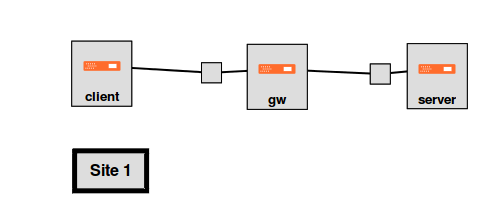
\includegraphics[width=14cm]{topologyGeni.png}
\caption{GENI Topology for Performance Evaluation}
\label{genitopo}
\end{figure}
Two different kinds of channel behavior are investigated: uniformly distributed on-off period and exponentially distributed on-off period. Congestion window size (CWND) and throughput are recorded to analyze the performance as in Figure \ref{1st}, \ref{2nd}, \ref{3rd} and \ref{4th}.  The channel capacity is set to be $1$Gbps. Figure \ref{1st} illustrates the CWND of the sender when the off period is exponentially distributed with mean $10ms$, $100ms$, $1s$, while Figure \ref{2nd} shows the corresponding throughput. Figure \ref{3rd} and \ref{4th} presents the CWND and throughput when the off period is uniformly distributed between $0ms - 10ms$, $0ms - 100ms$, $0ms - 1s$. In both cases, NewReno performance is deteriorated significantly due to the high frequency of off period. Figure \ref{1st}, \ref{3rd} showed every time off period happened, slow start will follow. The throughput is as low as $200$Mbps, which is $1/5$ of the full capacity. Compare with NewReno, from Figure \ref{1st}, \ref{3rd} we conclude that Cubic is more aggressive than NewReno. When channel recovers from off period to on period, Cubic will increase the CWND faster to utilize the channel capacity.  When channel off time is at the level of 10ms, cubic even did not notice there is a connection lost. Instead, it behaves as congestion happened in the network and reduce the CWND. When the on time period is long enough as in the exponentially on-off period case, Cubic can still reach the upper limit of CWND and achieve full throughput as in Figure \ref{2nd}, while NewReno needs more time to recover. In the uniformly distributed on-off period case, the channel lost happened before Cubic fully recovered as in Figure \ref{3rd}. The CWND has a descending trend and the throughput decreases as time goes on. Based on the aforementioned observation, we conclude that even Cubic will not achieve high throughput if the channel switch between LOS (on) and NLOS (off) with a high frequency. Therefore, an aggressive congestion control protocol is necessary for the 5G network. In the following sections, we will focus on the initial step of design this protocol: developing a fast end-user congestion prediction scheme.
\begin{figure}
\centering
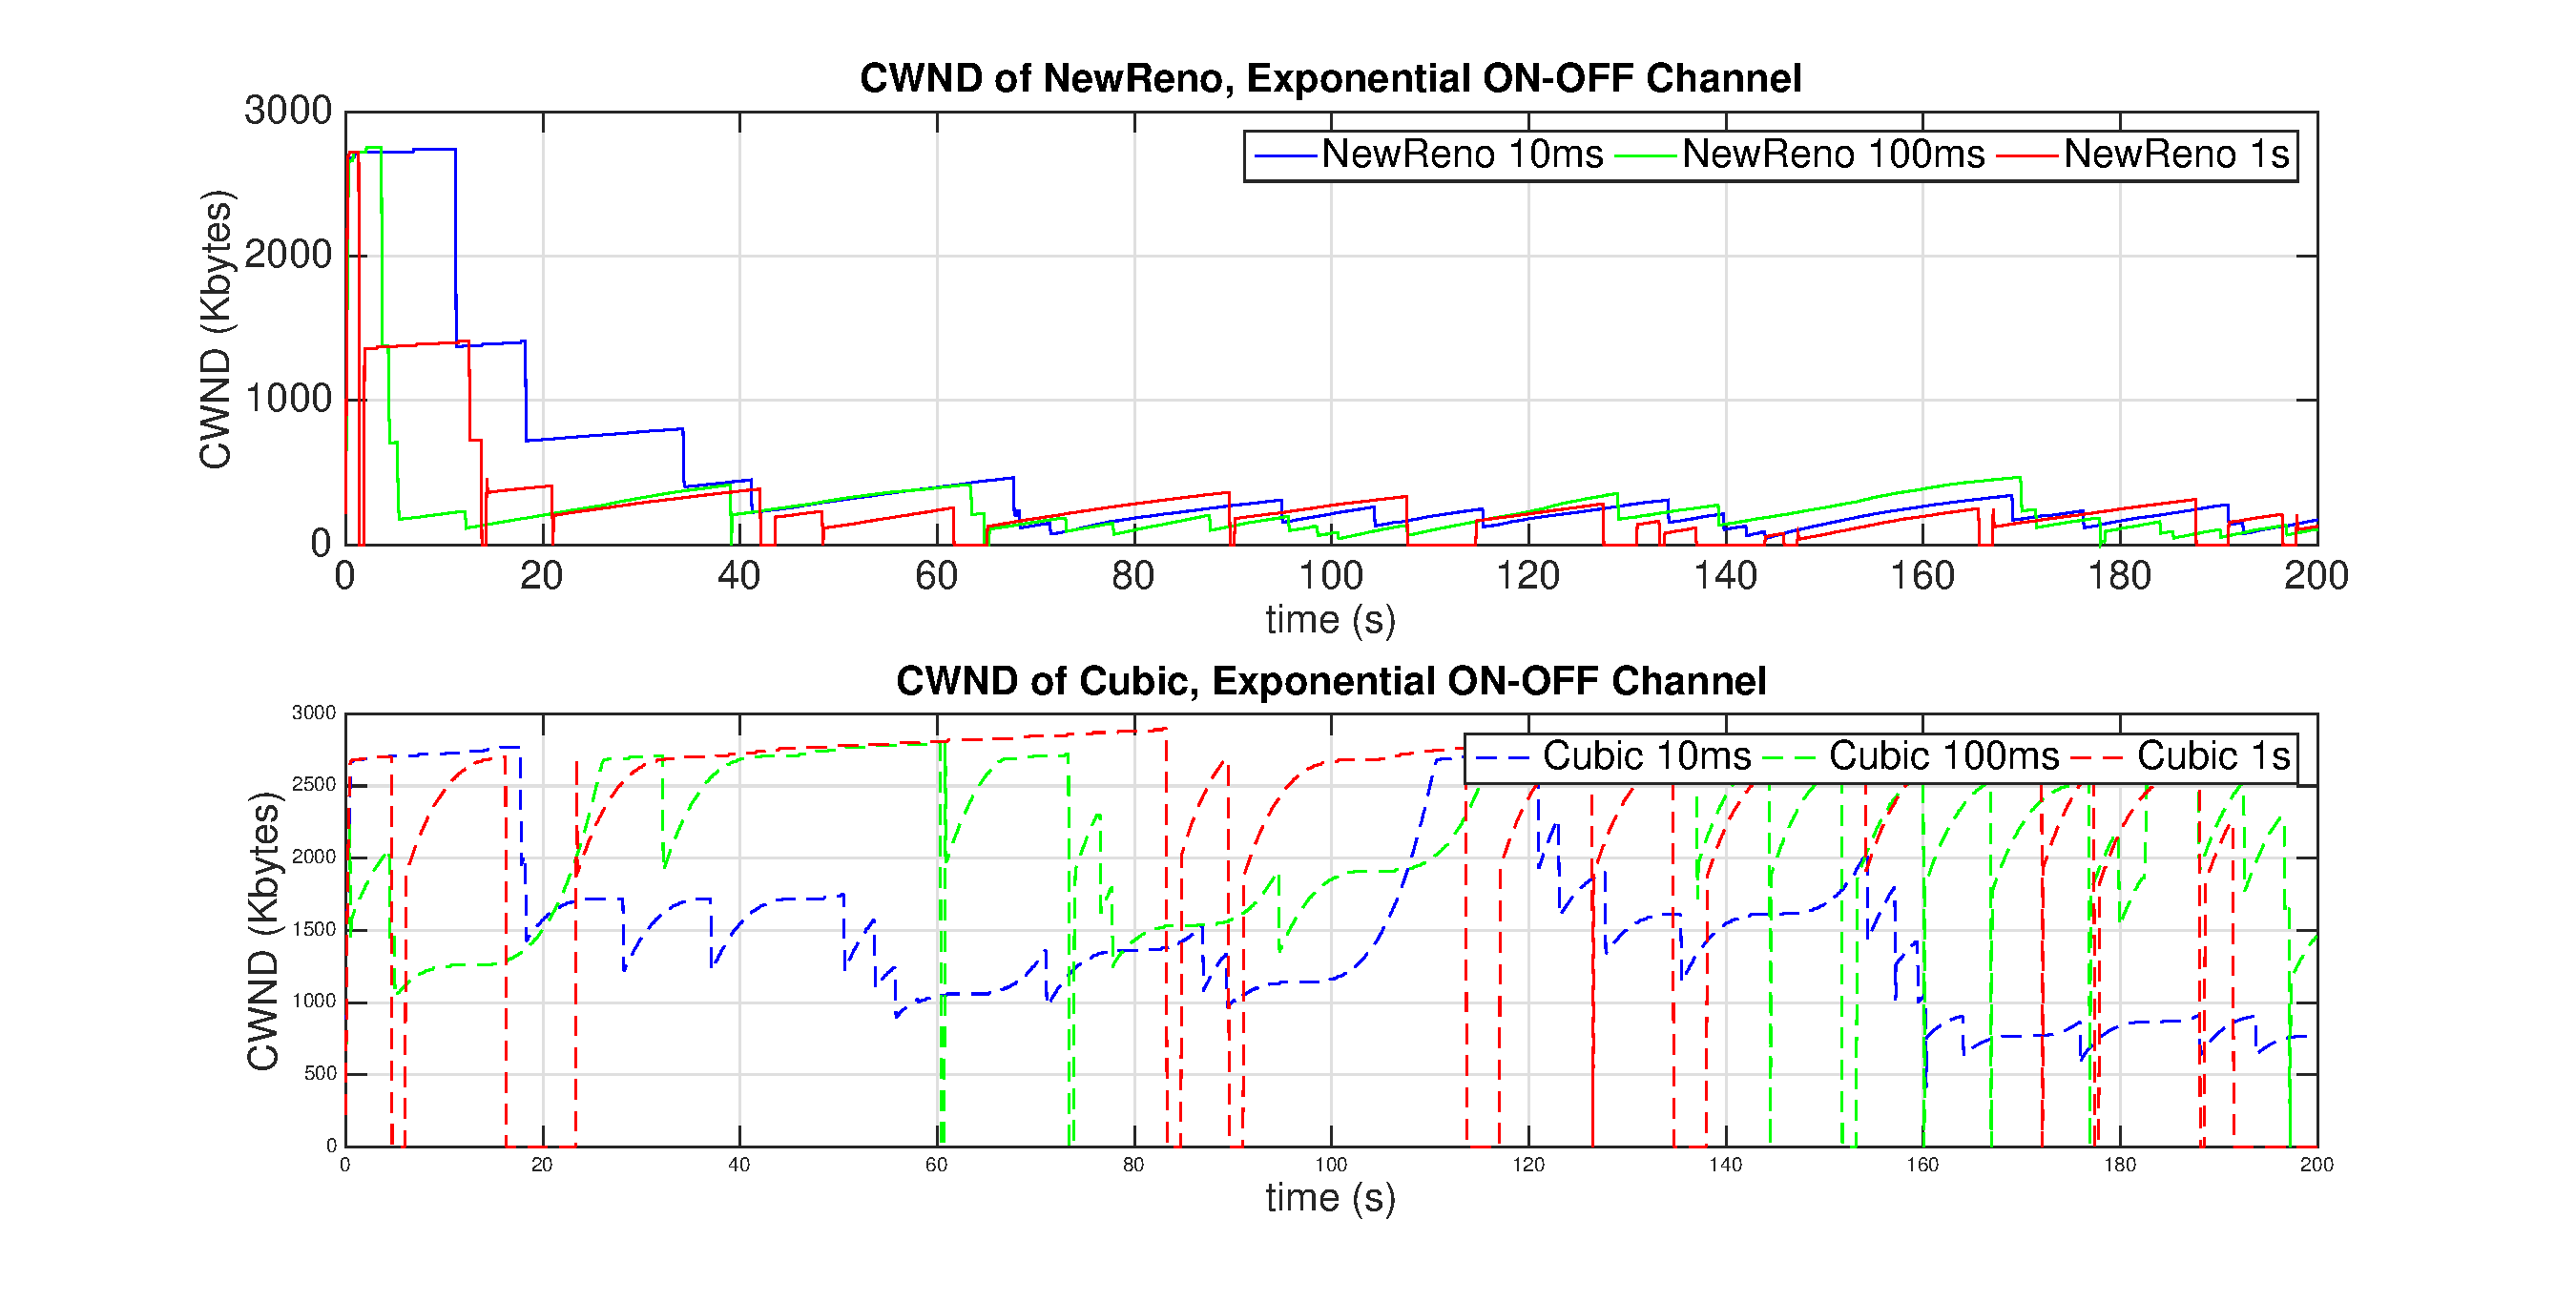
\includegraphics[width=14cm]{1.eps}
\caption{CWND dynamics given exponentially On-Off channel behavior}
\label{1st}
\end{figure}
\begin{figure}
\centering
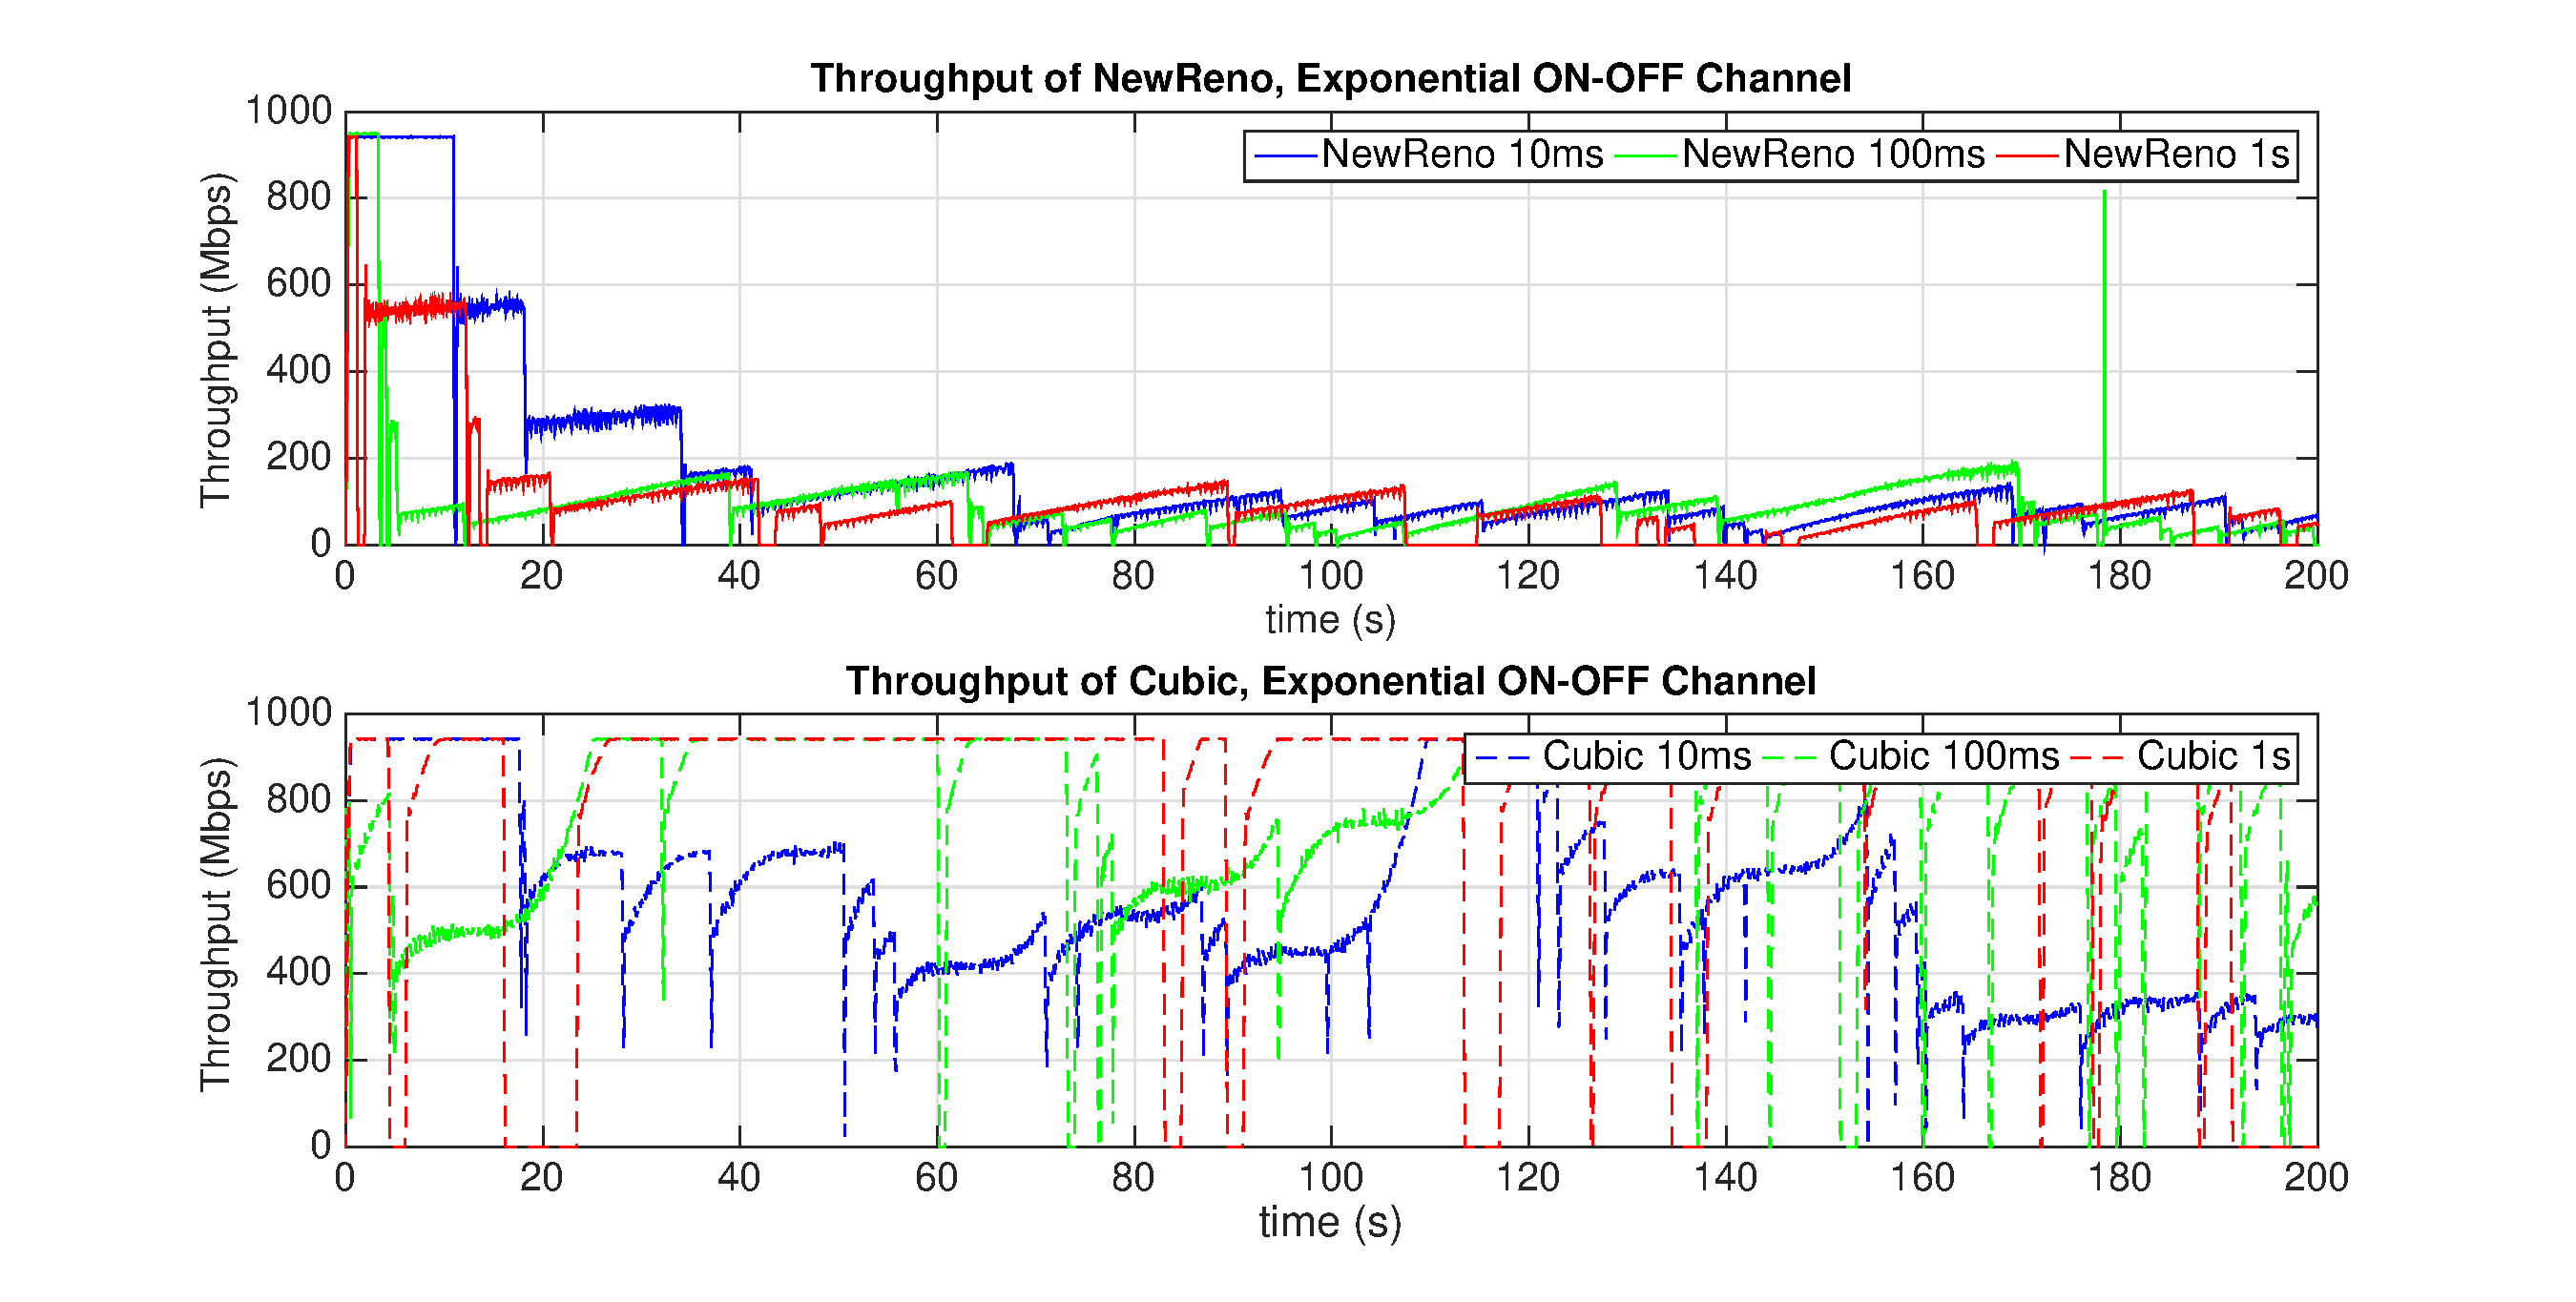
\includegraphics[width=14cm]{2.eps}
\caption{Throughput dynamics given exponentially On-Off channel behavior}
\label{2nd}
\end{figure}
\begin{figure}
\centering
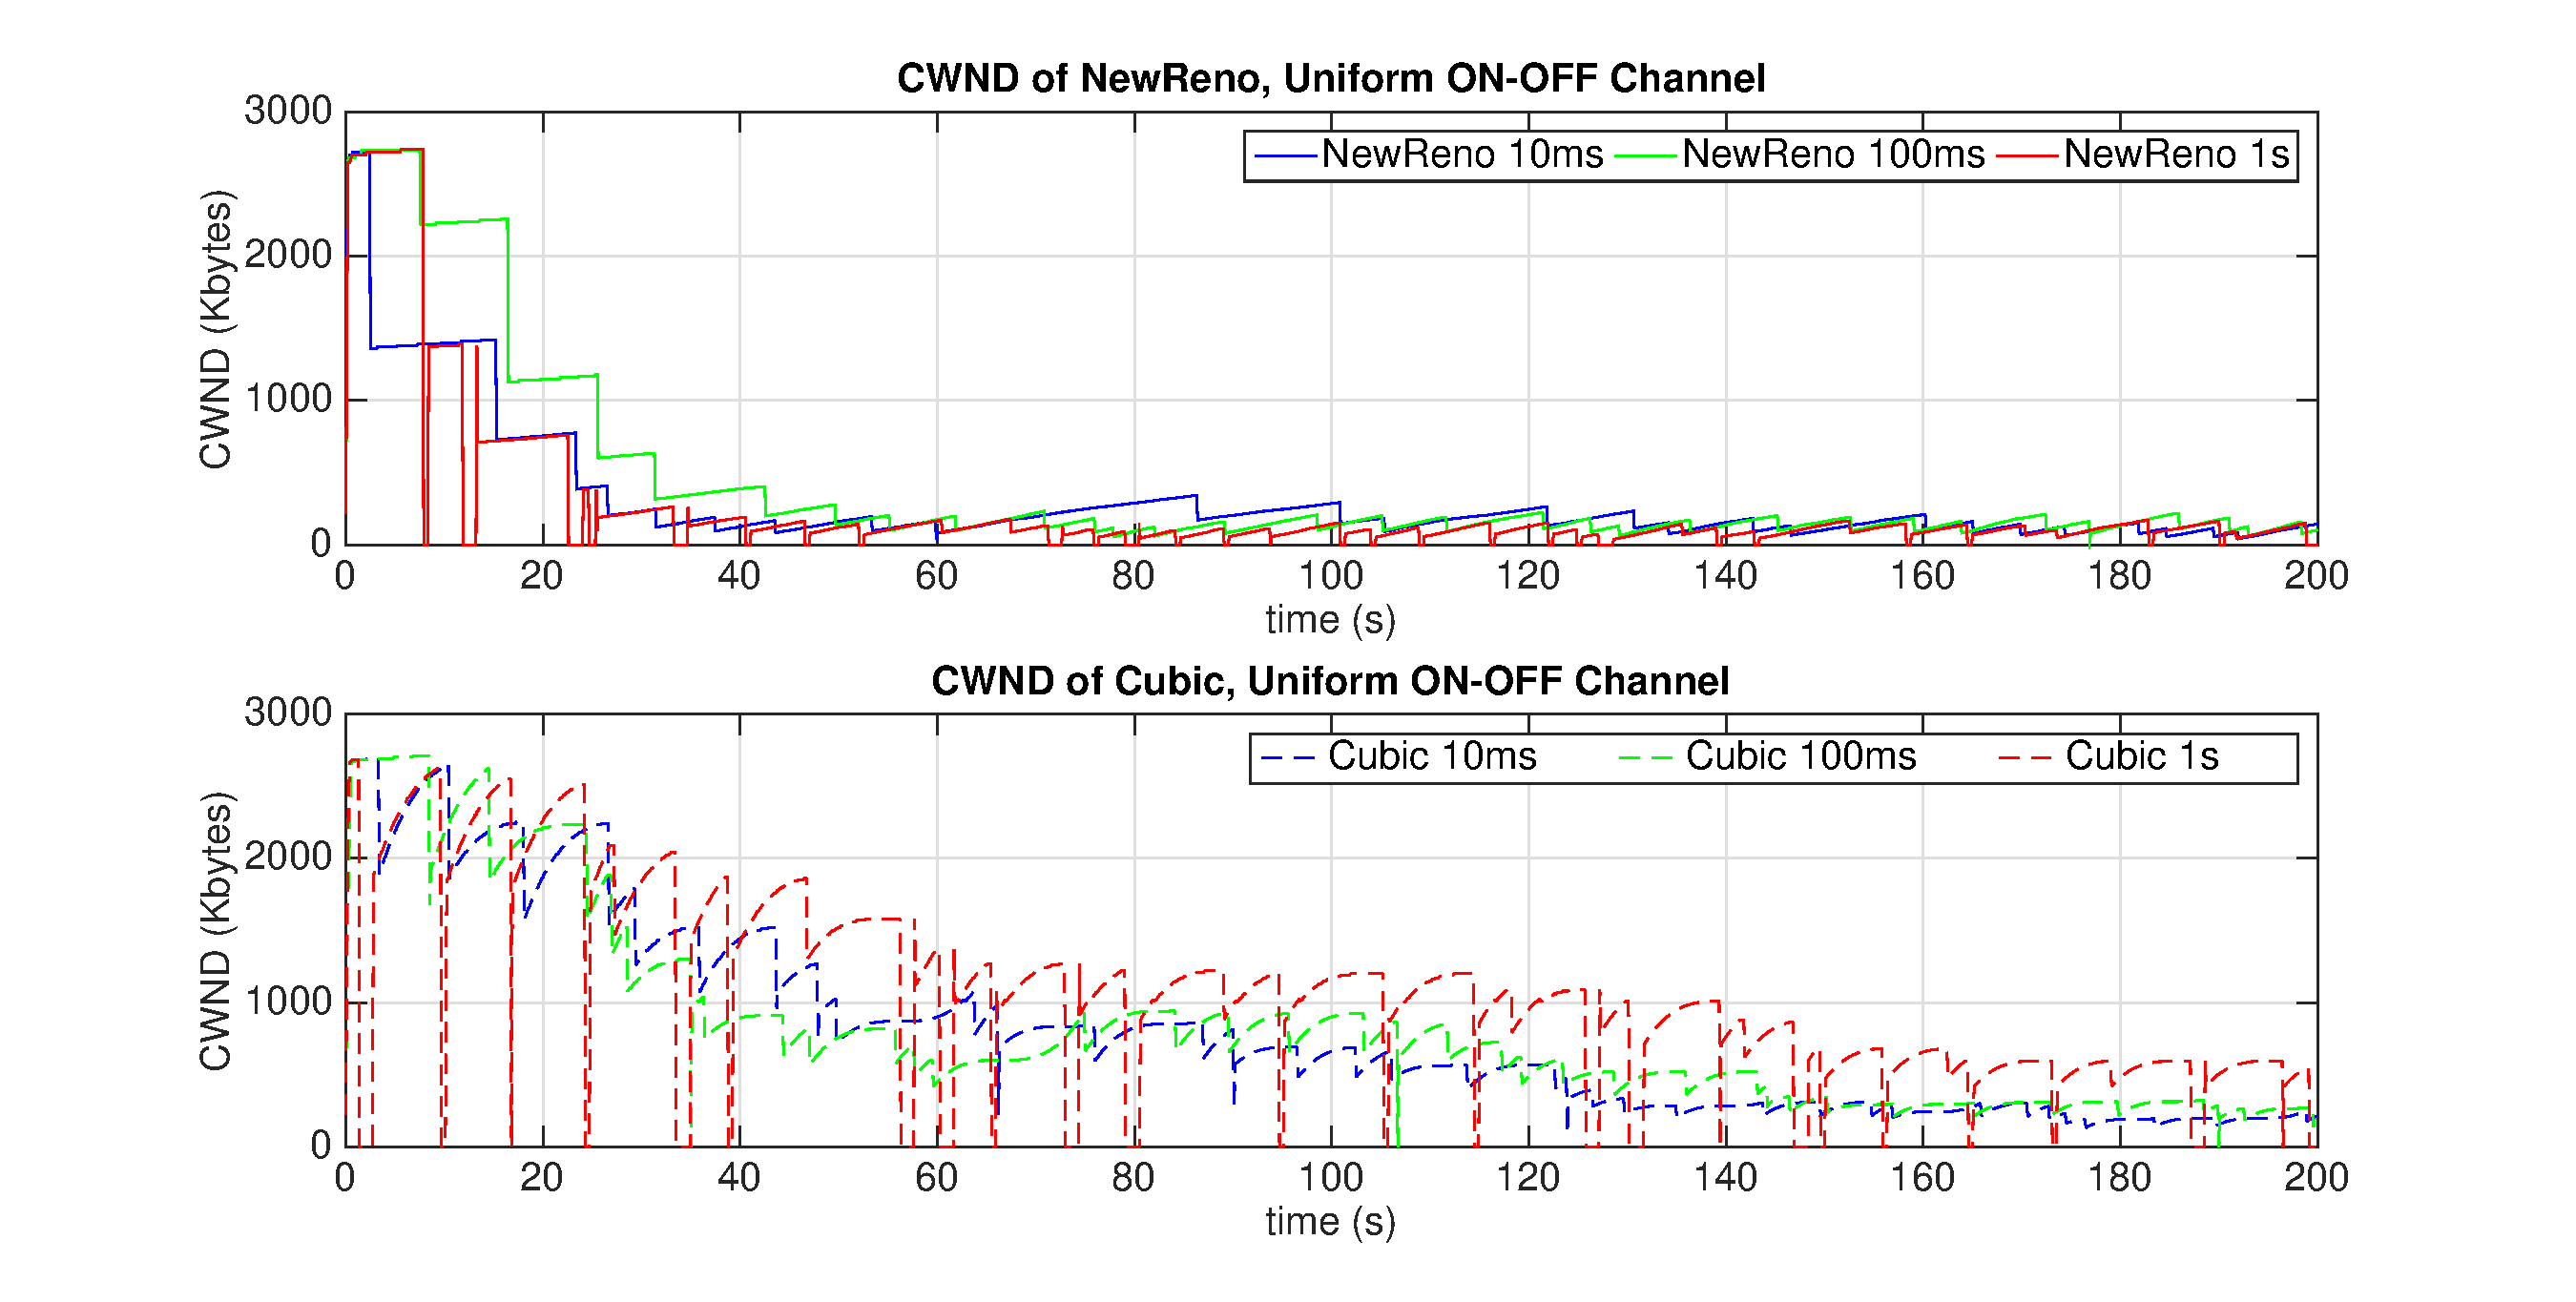
\includegraphics[width=14cm]{3.eps}
\caption{CWND dynamics given uniformly On-Off channel behavior}
\label{3rd}
\end{figure}
\begin{figure}
\centering
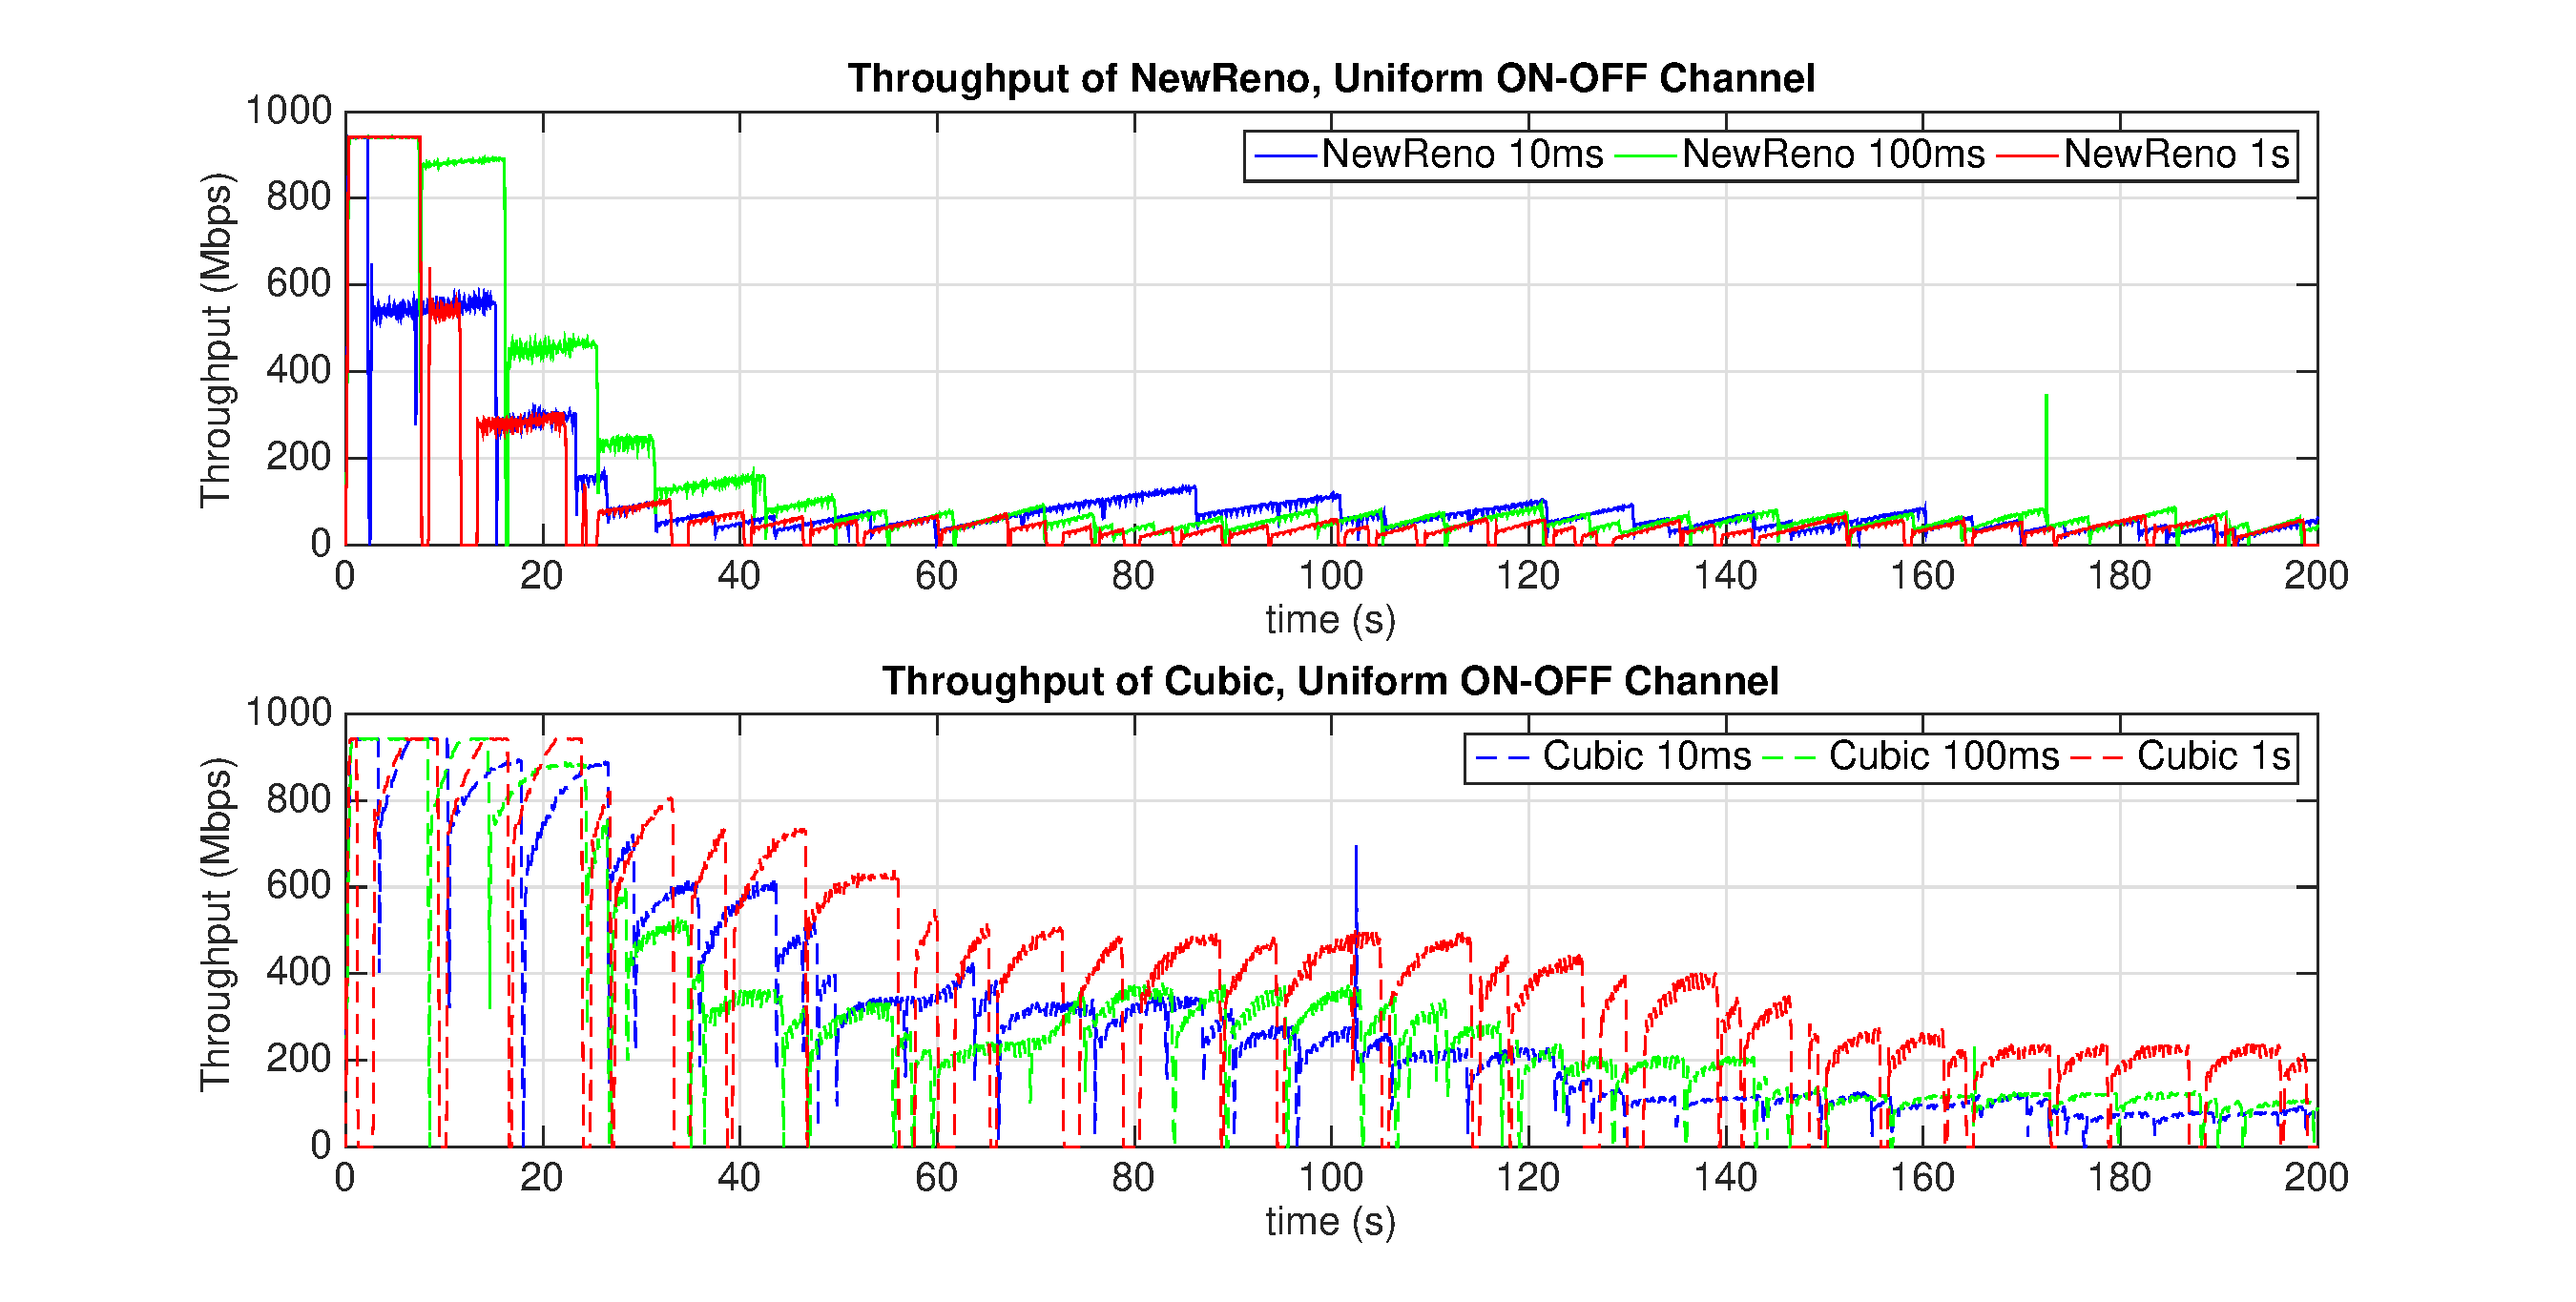
\includegraphics[width=14cm]{4.eps}
\caption{Throughput dynamics given uniformly On-Off channel behavior}
\label{4th}
\end{figure}
\section{Congestion Detection Algorithm}
\label{Design}
In this section, the design of the fast congestion detection algorithm is illustrated in detail. The principle idea is to predict the congestion in network within one inter-arrival time of ACKs from the end user data. The data which can be collected from end user includes packet sending time, ACK arriving time and the RTT calculated from these two time stamps. To collect these data for a particular network topology, we run simulations using discrete event based Network Simulator 2 (NS2). 
\subsection{Network Topology}
A typical dumbbell model is presented and used in this section. The network topology is as in Figure \ref{layout}. There are $6$ TCP traffic senders and $6$ receivers, sender $si$ sends data to receiver $ri$ through the bottleneck link $Q1\to Q2$. Both $Q1$ and $Q2$ maintain a DropTail Queue. The queue limit is set to be the bandwidth-delay product to ensure the full utilization of the link capacity.
%\begin{figure}[!htb]\centering
%   \begin{subfigure}{0.49\textwidth}
%     \frame{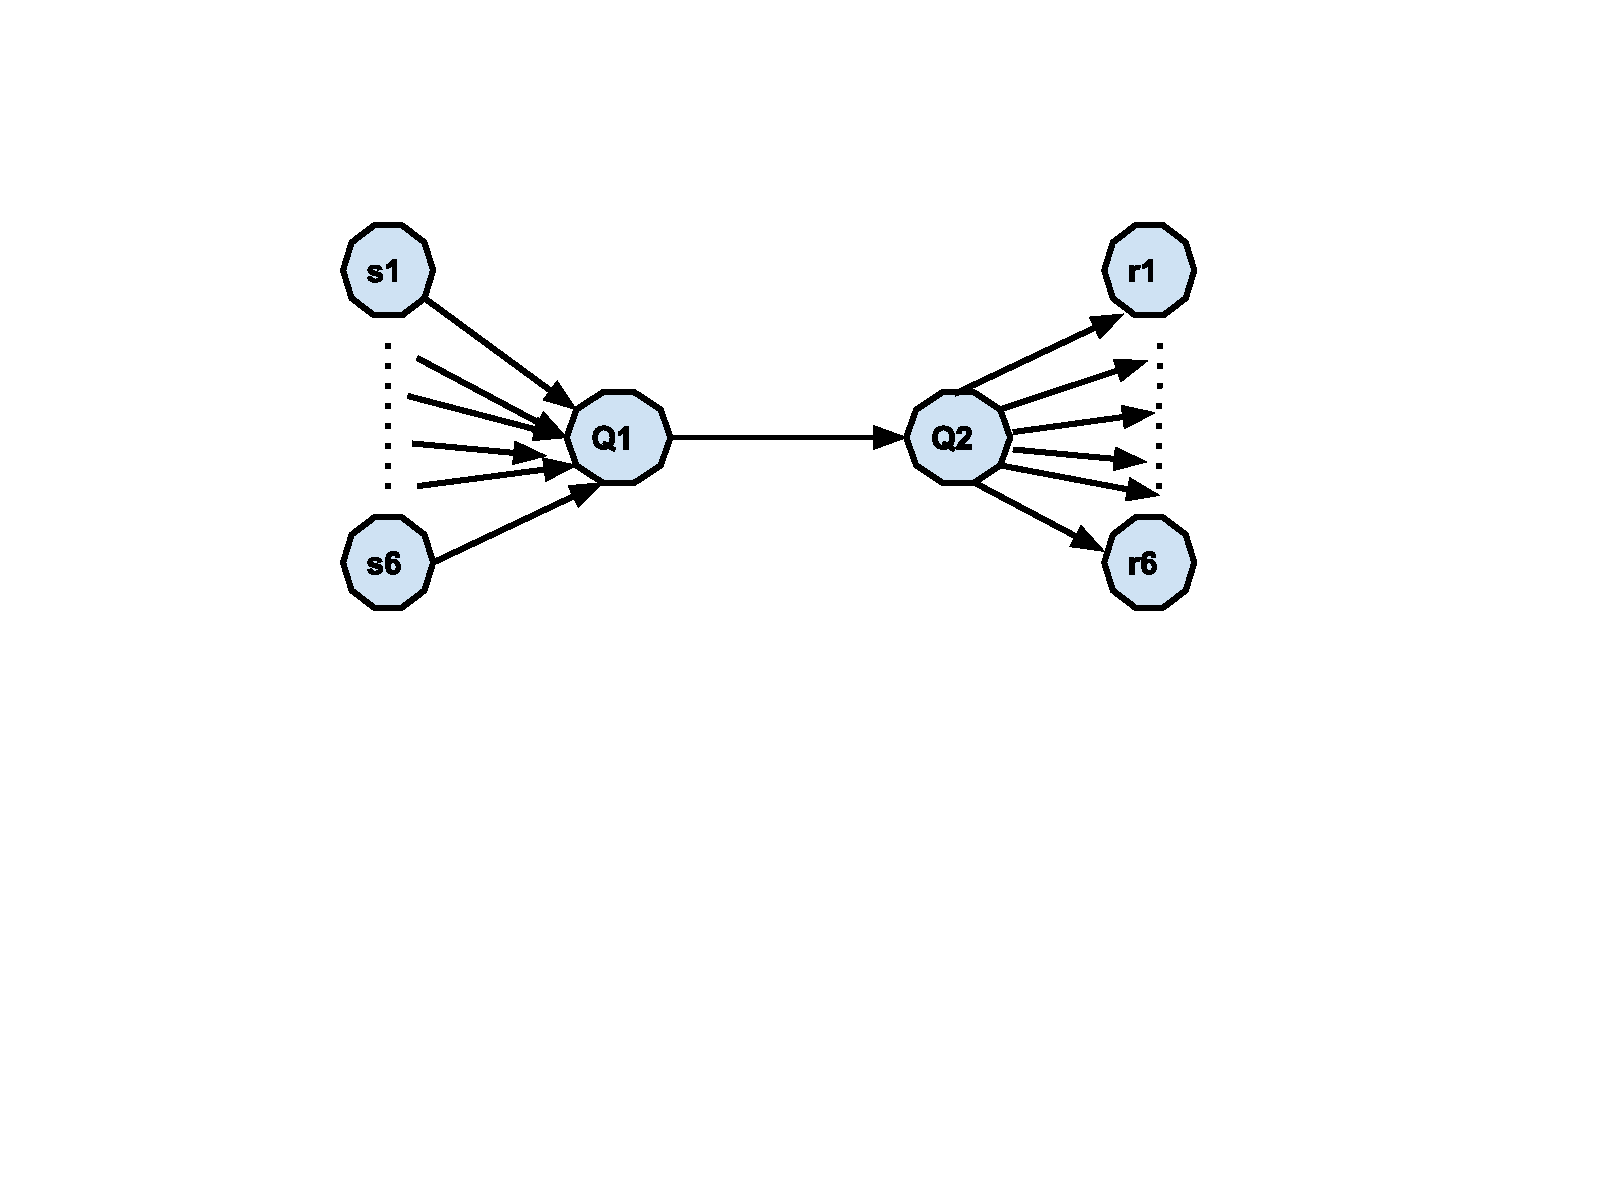
\includegraphics[width=6cm]{6layout.pdf}}
%     \caption{Network Topology}\label{layout}
%   \end{subfigure}
%   \begin {subfigure}{0.49\textwidth}
%     \frame{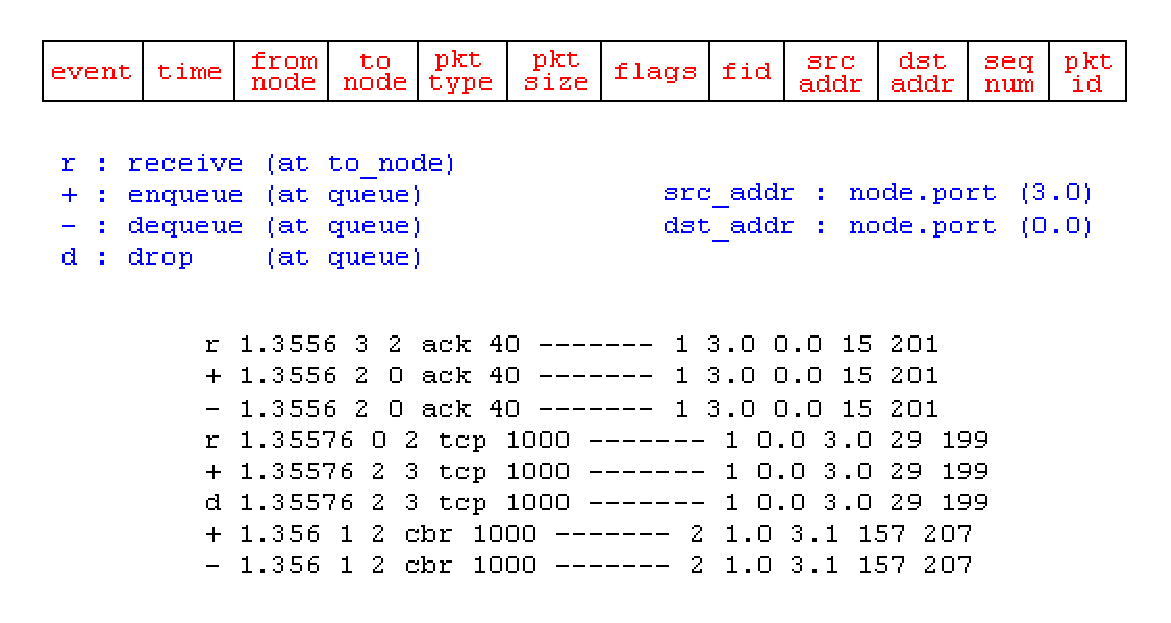
\includegraphics[width=6cm]{format.eps}}
%     \caption{NS2 TCP Trace Format}\label{NS2Format}
%   \end{subfigure}
%\end{figure}

\begin{figure}
\centering
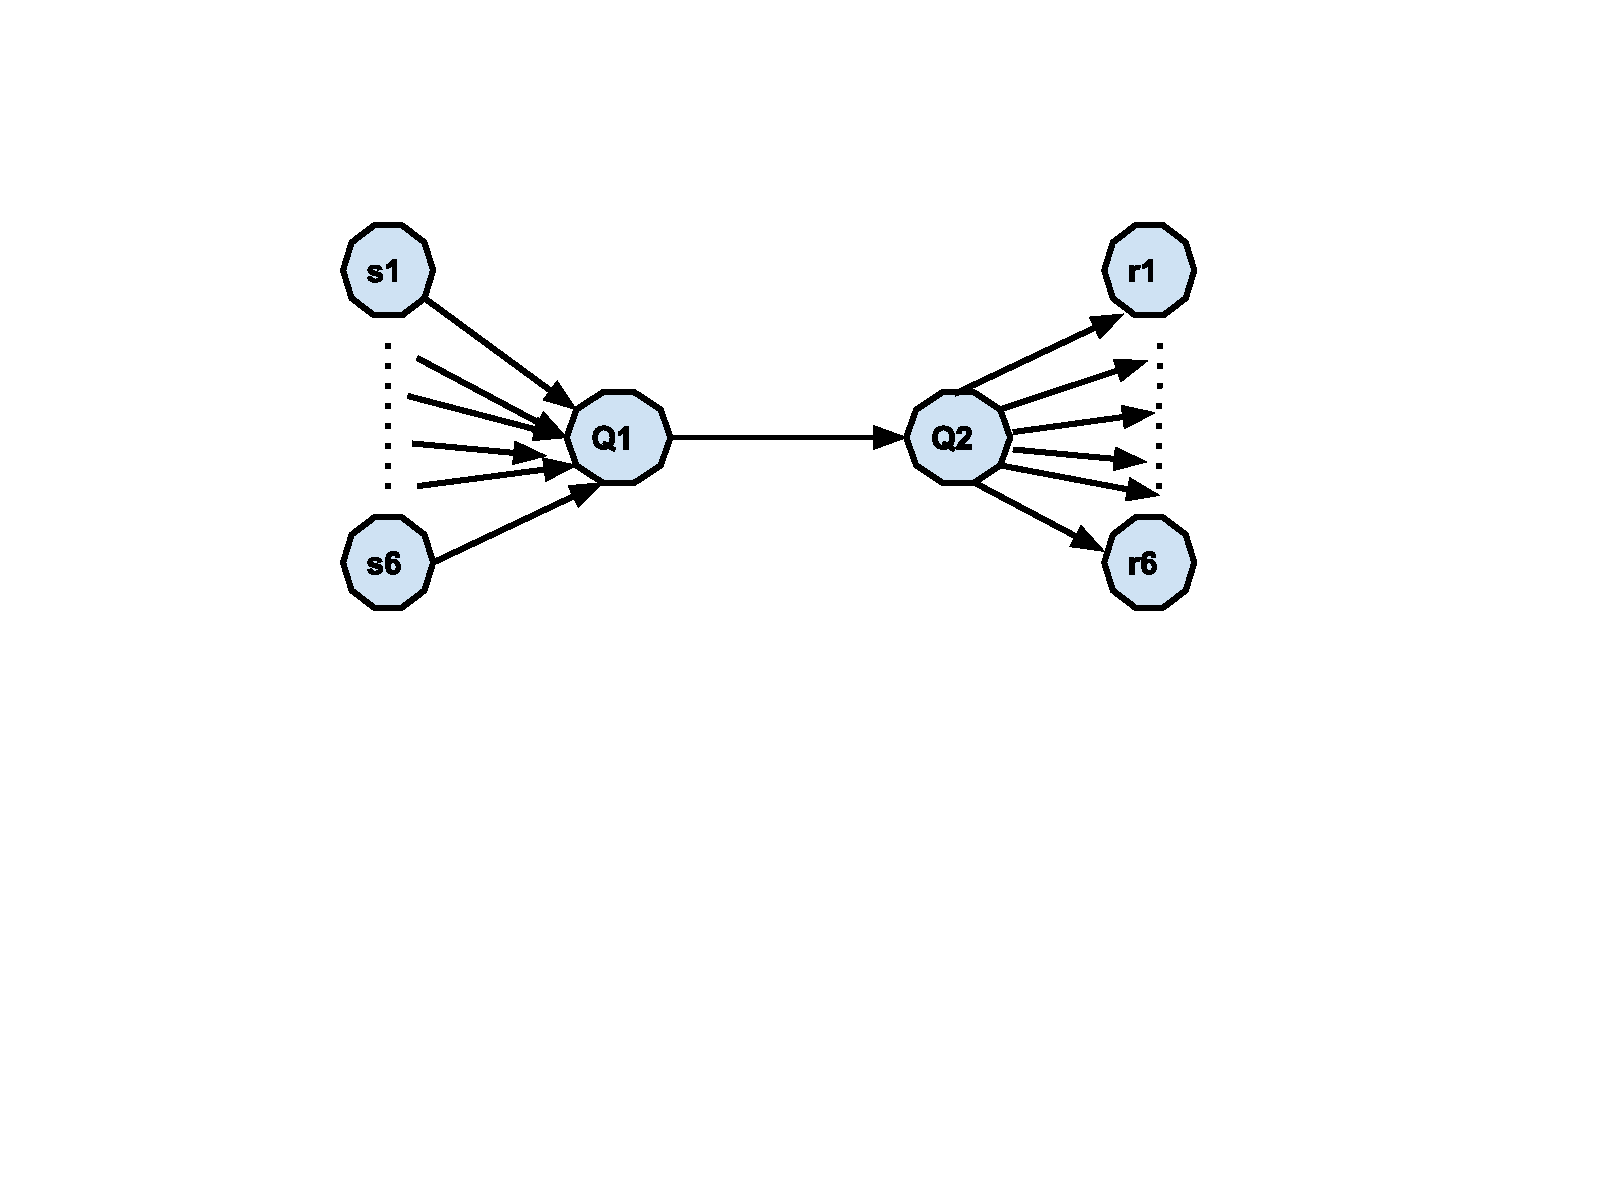
\includegraphics[width=10cm]{6layout.pdf}
\caption{Network topology}
\label{layout}
\end{figure}
Congestion occurs when the occupied queue length exceeds the threshold $T$ on the arriving of the incoming packet. To generate traces with congestion identifiers, we mark every packet as Congestion Experienced in the queue when the queue length is greater than $T$. Typical NS2 TCP traces  \cite{TraceFormat} are collected for future data processing as in Figure \ref{NS2Format}. 

\begin{figure}
\centering
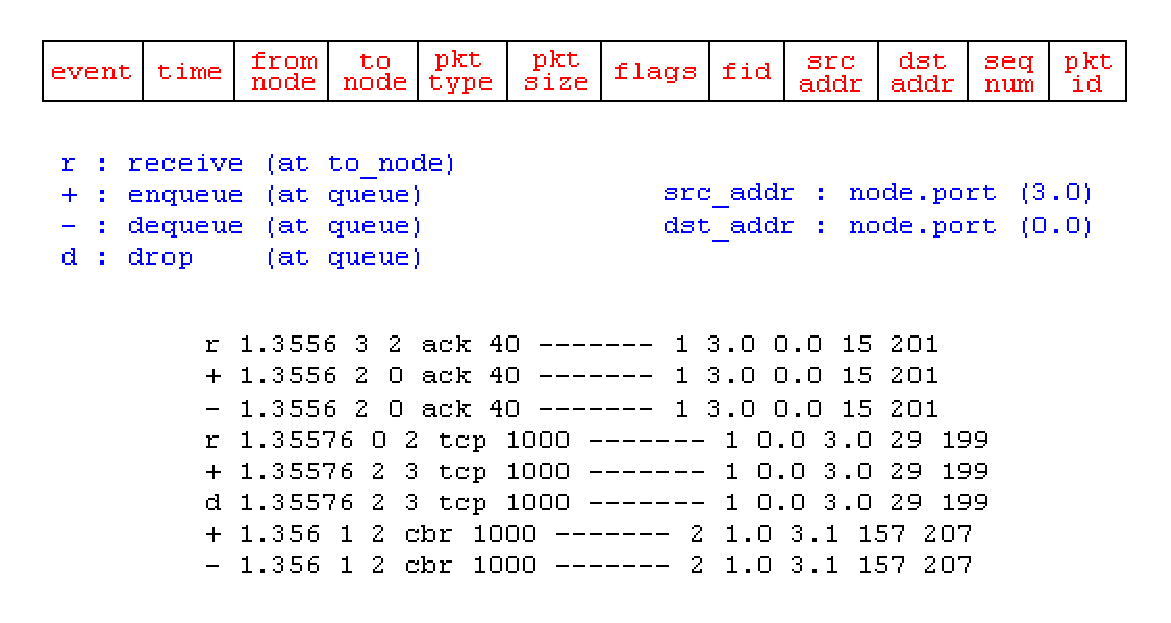
\includegraphics[width=10cm]{format.eps}
\caption{NS2 TCP trace format}
\label{NS2Format}
\end{figure}
From the trace format we can identify the packet sending time, arriving time, packet size, unique ID, etc. Matching the packet unique ID, RTT can be calculated from packet sending time and corresponding ACK receiving time. For each unique packet, if congestion happens upon its arriving, the unique ID was recorded to be Congestion Experienced.

\par The drop tail queue behavior is displayed as follows.
% Figure \ref{queuelengthCubic}
% and Figure \ref{queuelengthNewRenoVSUDP} are two different queue behavior patterns. 
Figure \ref{queuelengthCubic} shows queue changes when traffic sources are running Cubic TCP with UDP competing traffic. 
%while Fig. \ref{queuelengthNewRenoVSUDP} shows the case one part of traffic sources are running NewReno TCP with competing UDP traffic.
In this case, when queue length is greater than $450$ packets, the incoming packets will be marked as congestion experienced.

%\begin{figure}
%\includegraphics[width=8cm]{queue.eps}
%\caption{Queue Length Dynamics (NewReno)}
%\label{queuelengthNewReno}
%\end{figure}
%\begin{figure}[!htb]\centering
%   \begin{subfigure}{0.49\textwidth}
%     \frame{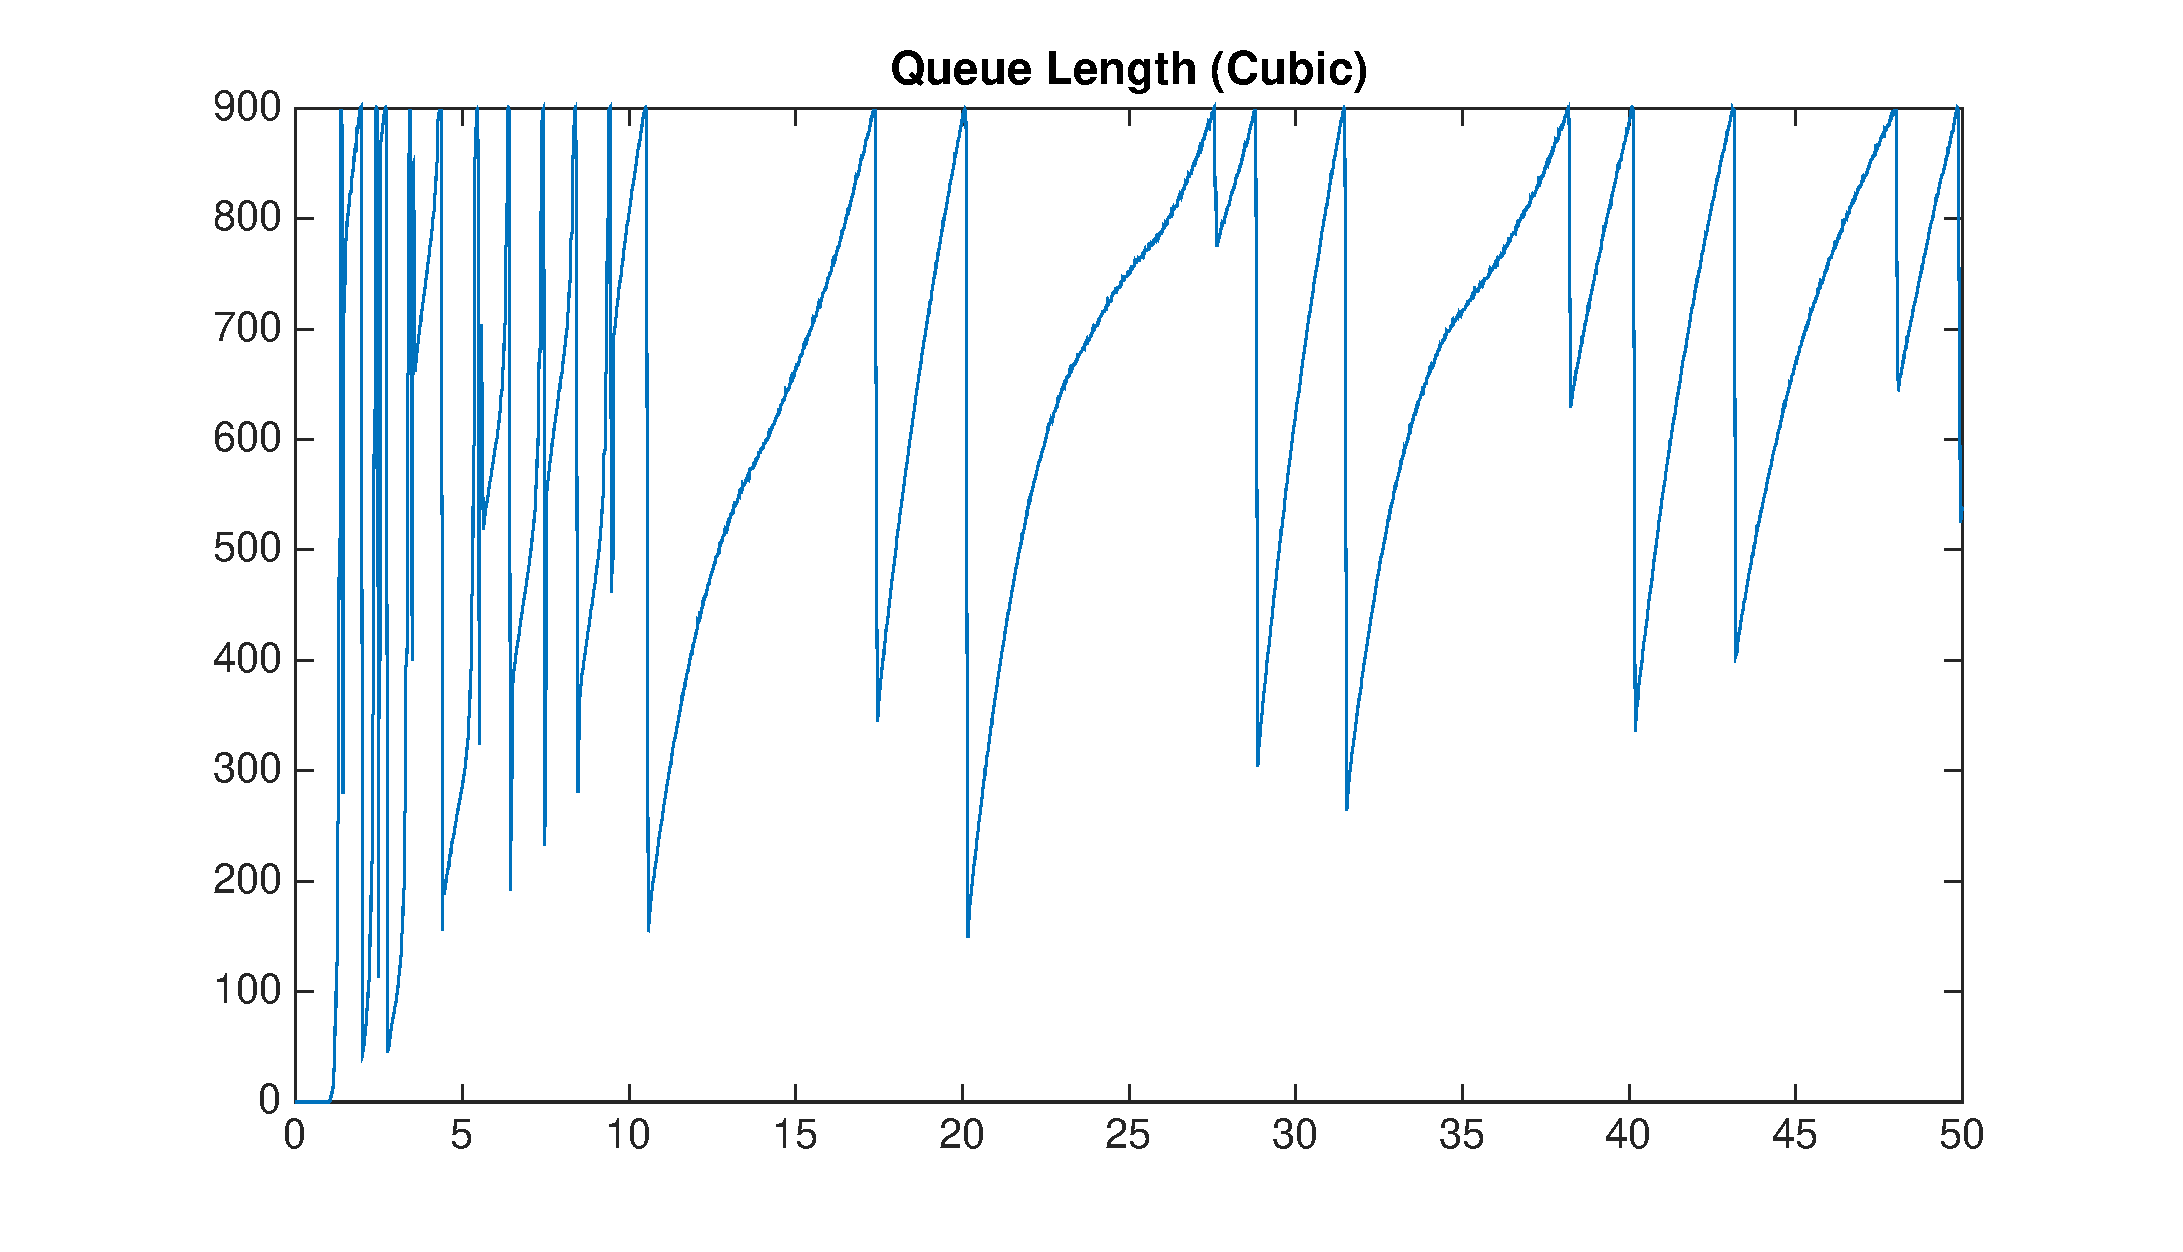
\includegraphics[width=6cm]{QueueLengthCubic.eps}}
%     \caption{Queue Length (Cubic)}
%\label{queuelengthCubic}
%   \end{subfigure}
%   \begin {subfigure}{0.49\textwidth}
%     \frame{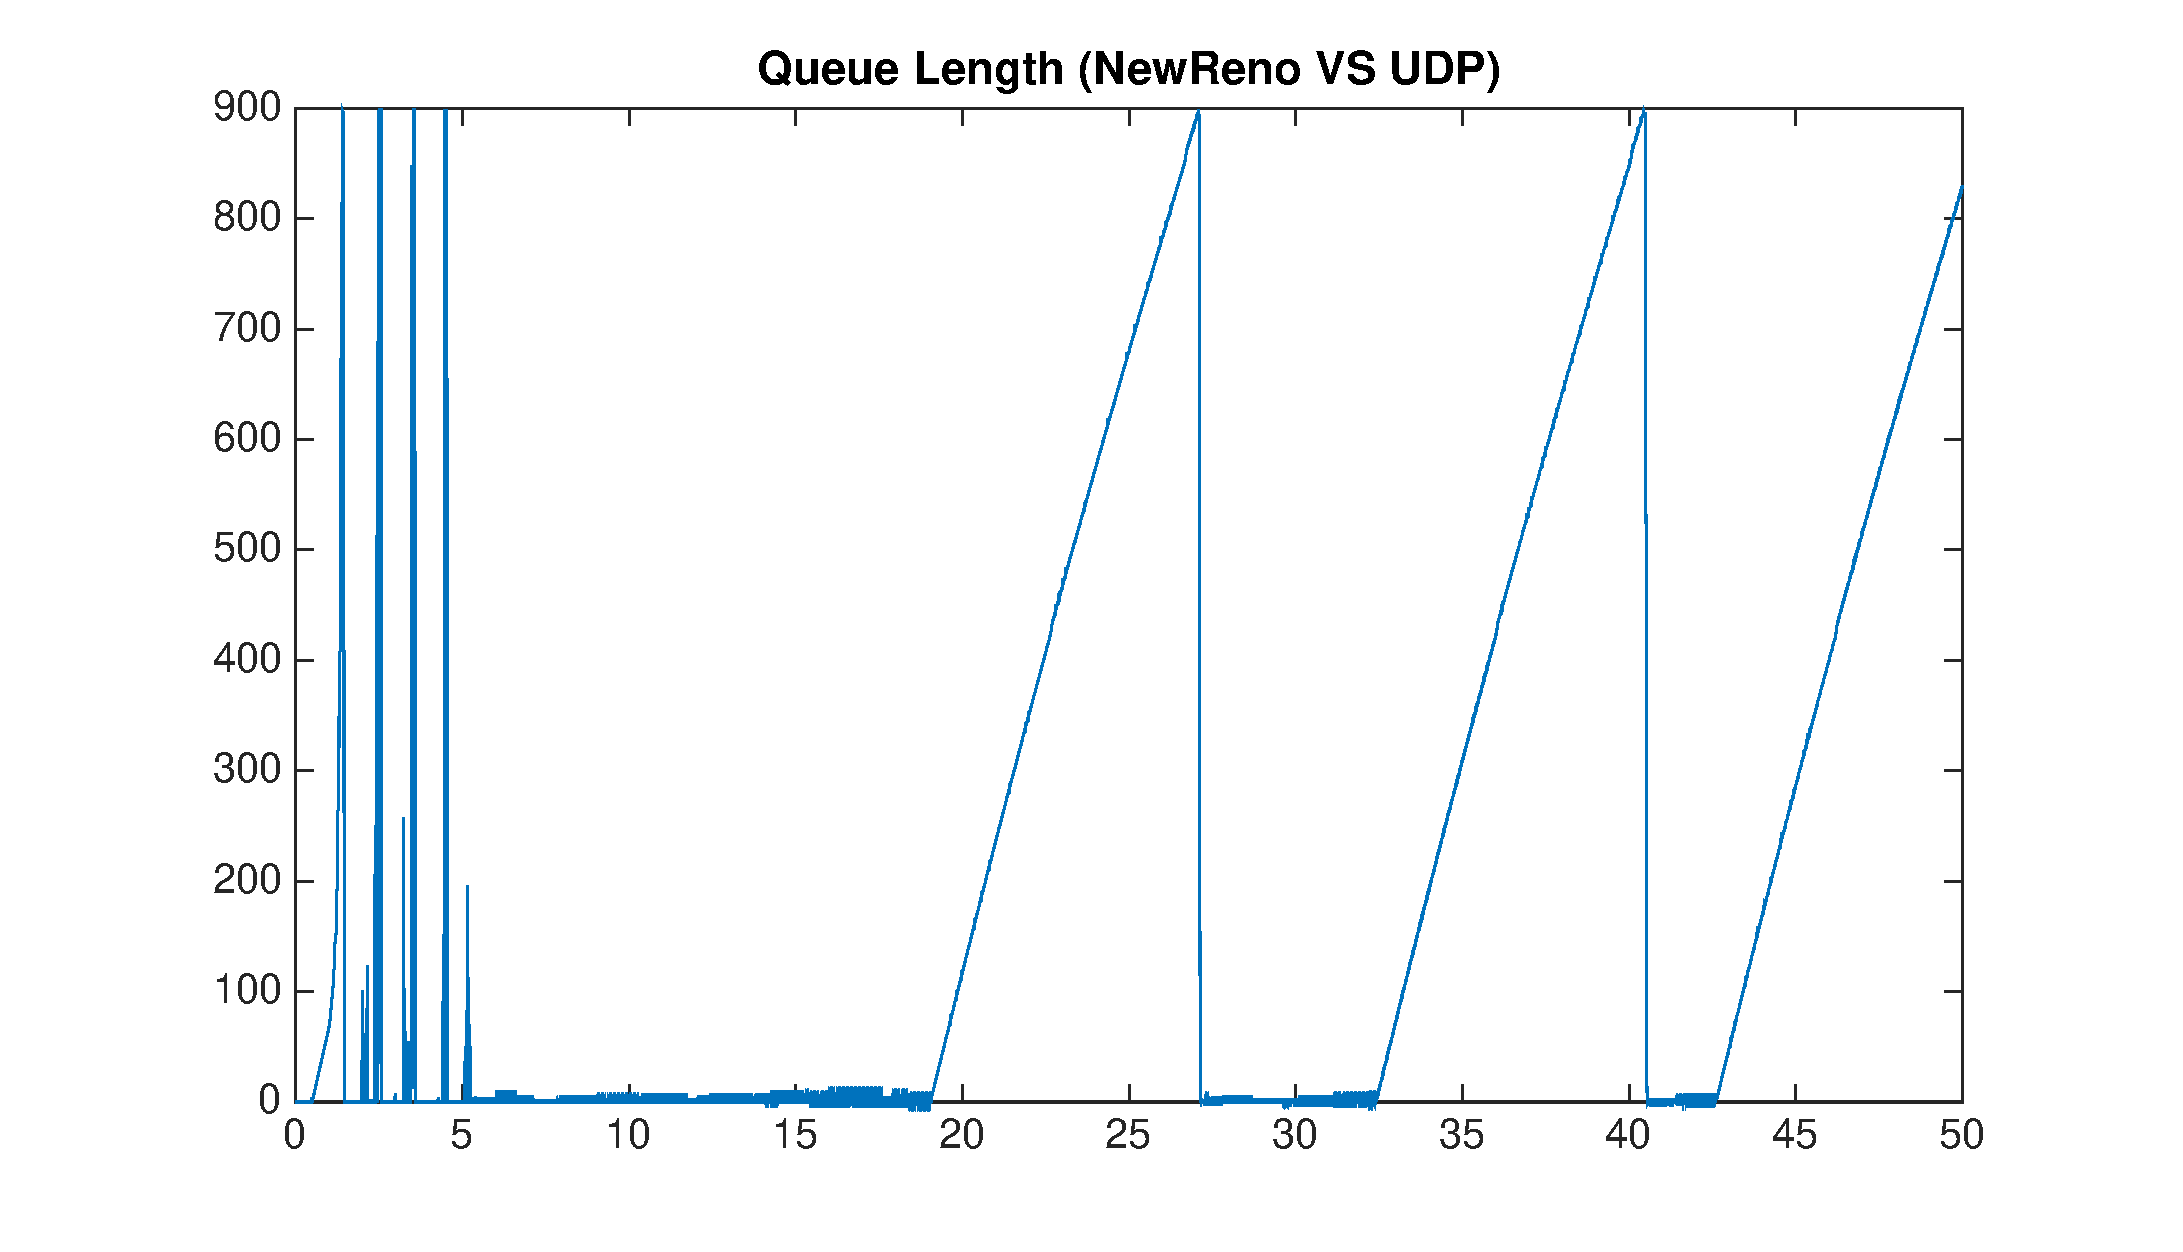
\includegraphics[width=6cm]{QueueLengthNewRenoVSUDP.eps}}
%   \caption{Queue Length (NewReno VS UDP)}
%\label{queuelengthNewRenoVSUDP}
%   \end{subfigure}
%\end{figure}

\begin{figure}
\centering
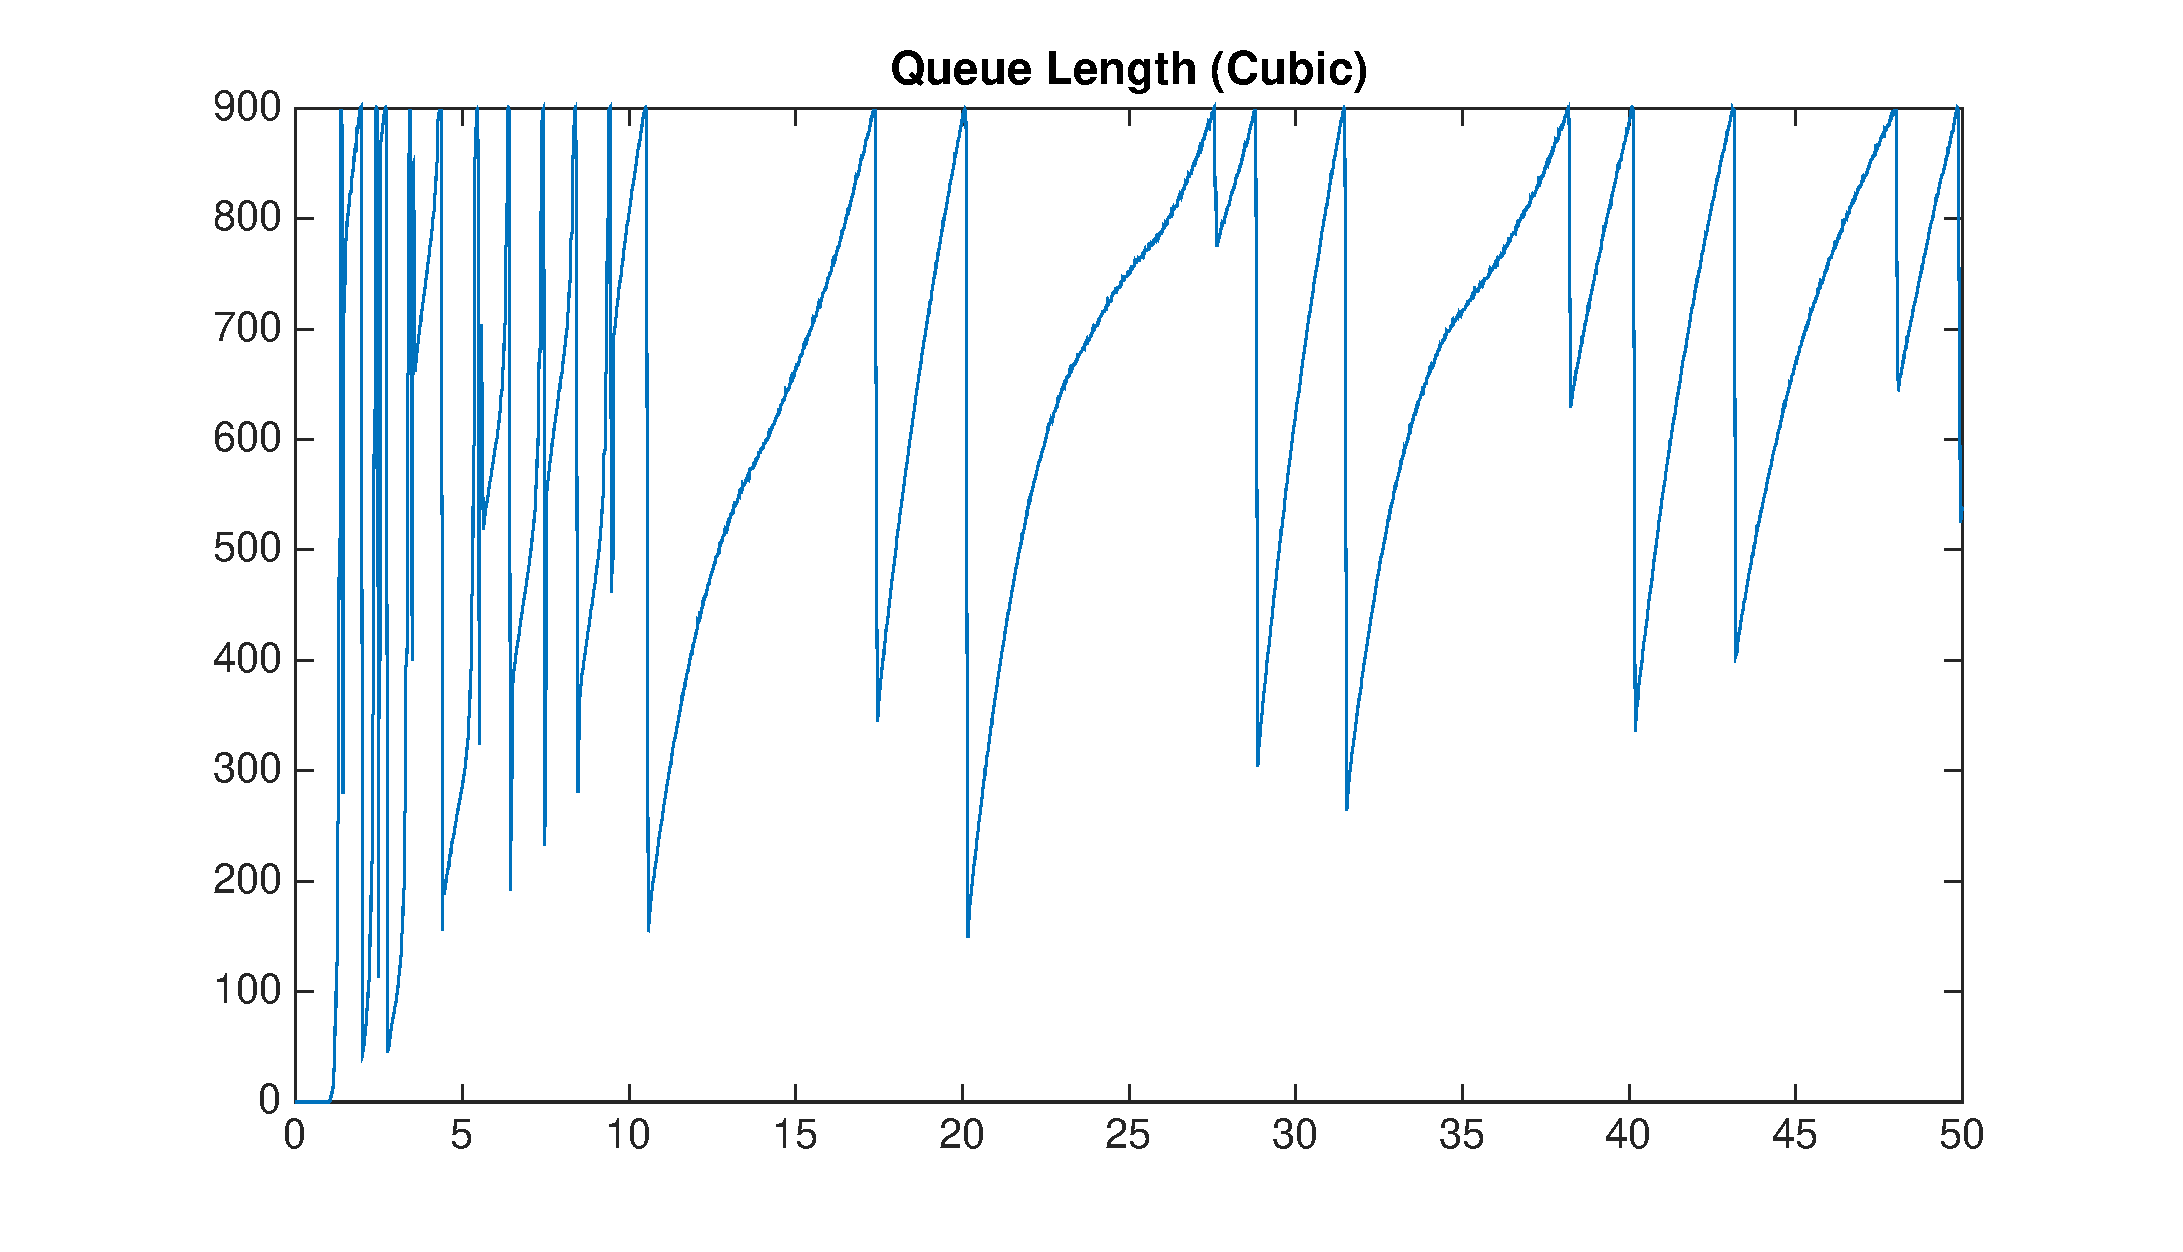
\includegraphics[width=10cm]{QueueLengthCubic.eps}
\caption{Queue length dynamics (Cubic)}
\label{queuelengthCubic}
\end{figure}

%\begin{figure}
%\centering
%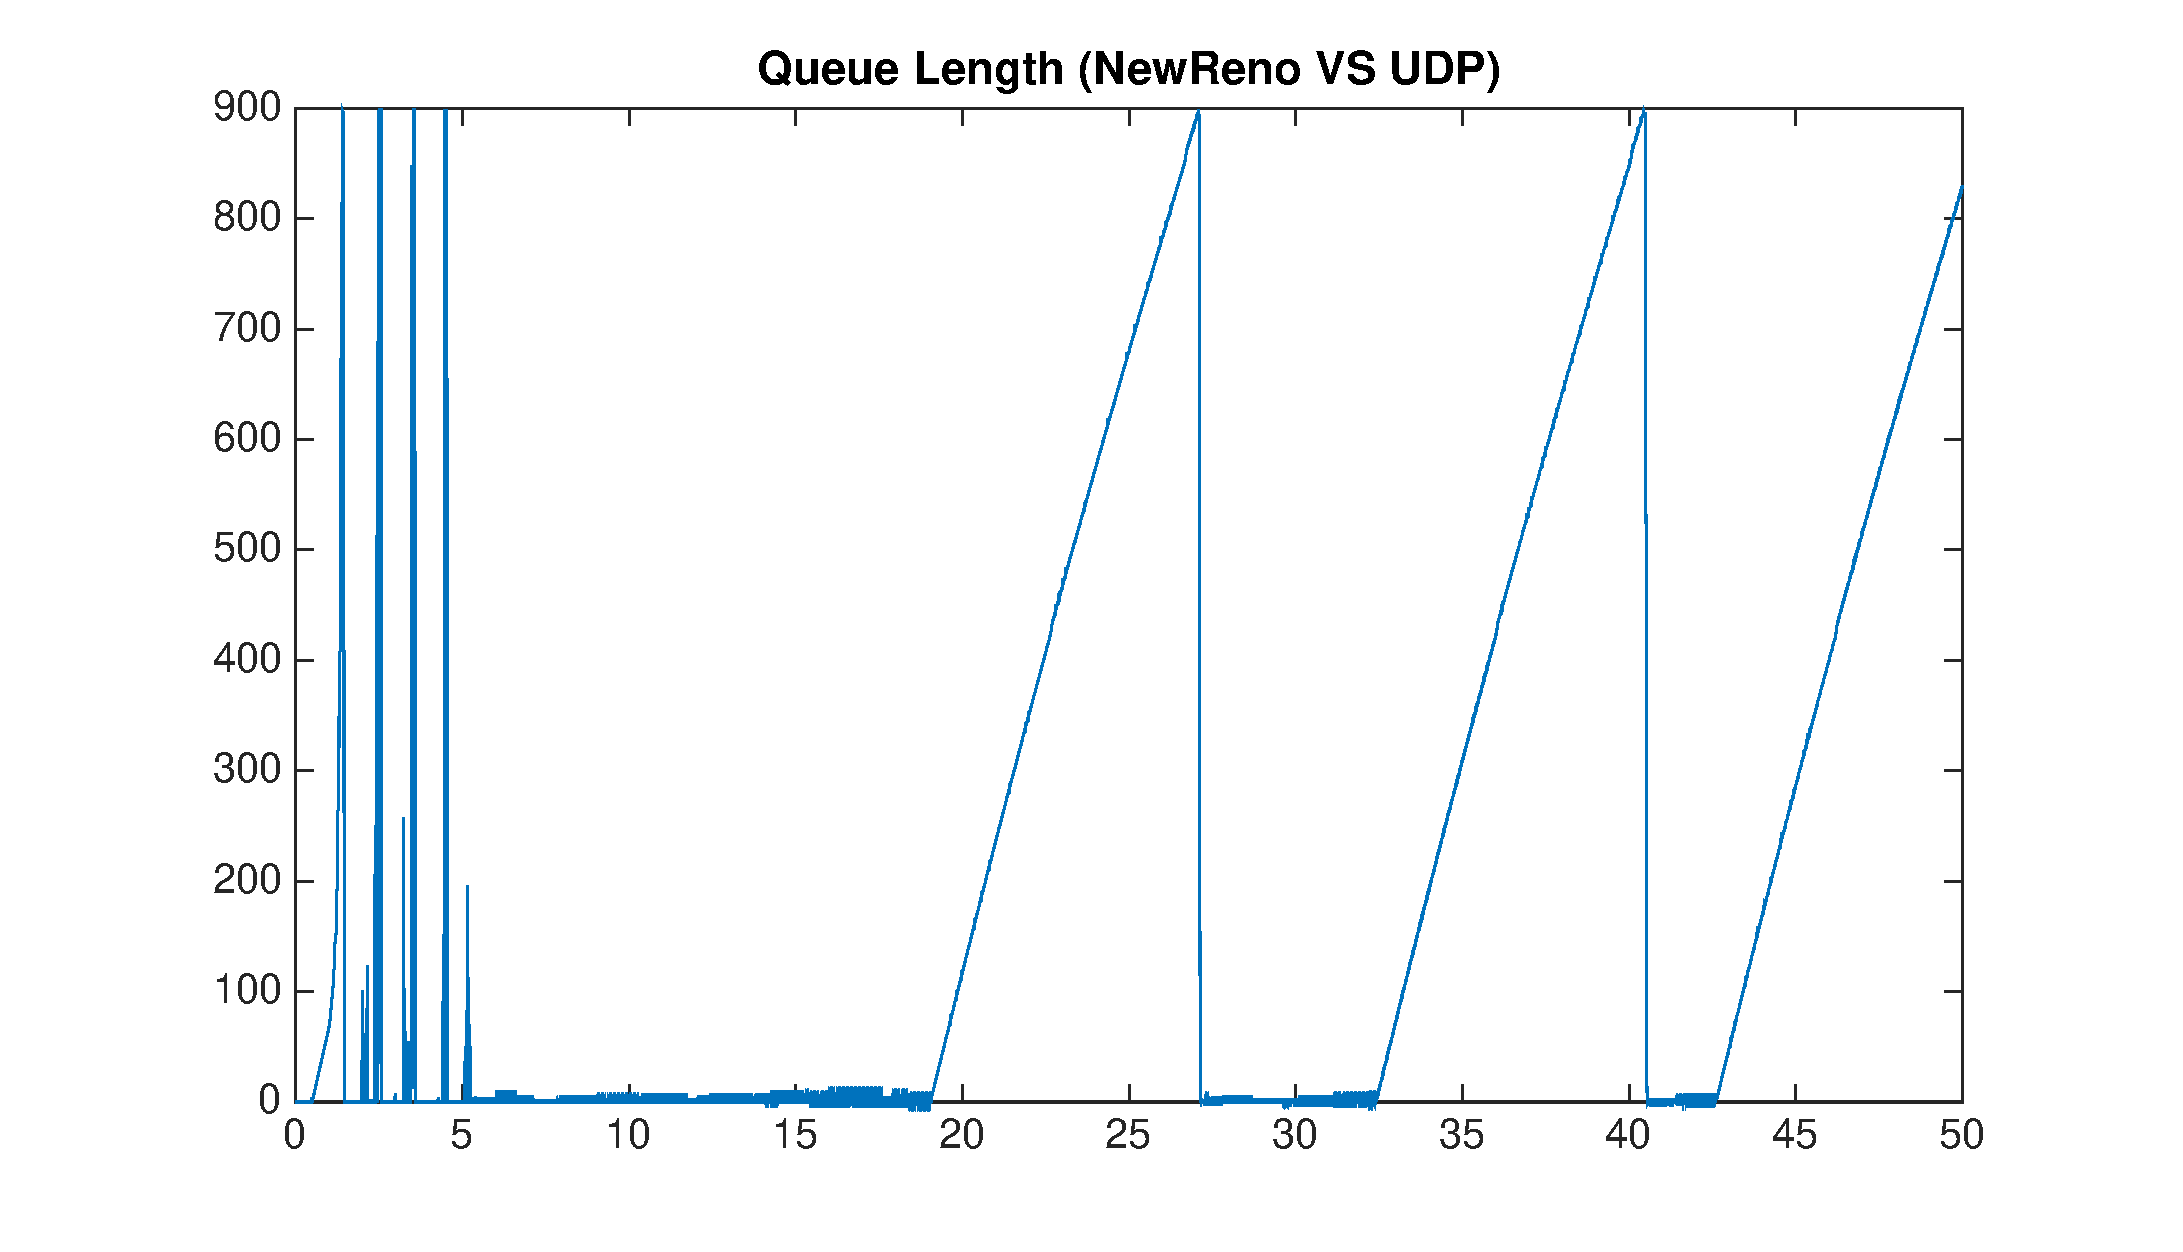
\includegraphics[width=10cm]{QueueLengthNewRenoVSUDP.eps}
%\caption{Queue Length Dynamics (NewReno VS UDP)}
%\label{queuelengthNewRenoVSUDP}
%\end{figure}

\subsection{Data Collection}
Without losing generality of the analysis, we simulated several different traffic scenarios to collect end user data. We investigated following scenarios: 
\begin{itemize}
    \item Scenario 1: All traffic sources are running TCP NewReno with stationary bottleneck link capacity.
    \item Scenario 2: All traffic sources are running TCP Cubic with stationary bottleneck link capacity.
    % \item Scenario 3: One half traffic sources are running TCP NewReno while the other half running TCP Cubic with stationary bottle link capacity.
    \item Scenario 3: One half of traffic sources are running TCP NewReno while the other half are running UDP with stationary bottleneck link capacity.
    \item Scenario 4: One half of traffic sources are running TCP Cubic while the other half are running UDP with stationary bottleneck link capacity.
    \item Scenario 5: Repeat scenario 1 and 2 for a periodically On-Off bottleneck link.
\end{itemize}
The bottleneck link for those scenarios is link $Q1 \to Q2$. Detailed simulation parameters are shown in TABLE \ref{tab:simuPara}.

\par The data which is available from end user are packet sending time $t_{s}$ and ACK receiving time $t_{r}$. From these two timestamps, we can calculate packet sending interval $T_{s_{i}} = t_{s_{i}} - t_{s_{i-1}}$, ACK inter-arrival time $T_{r_{i}} = t_{r_{i}} - t_{r_{i-1}}$ and Round Trip Time (RTT) $RTT_{i} = t_{s_{i}} - t_{r_{i}}$. From the above three available time intervals, we develop 5 features that are used in the congestion prediction algorithm.
\begin{table}
\begin{center}
\caption {Simulation Parameters} \label{tab:simuPara}
\begin{tabular}{ |c|c| }
 \hline
 Access Link Capacity & 1Gbps  \\
 \hline
 BottleNeck Link Capacity & 1Gbps  \\
 \hline
 Access Link Delay & 5ms  \\
 \hline
 BottleNeck Link Delay & 10ms\\
 \hline
 Queue Capacity & Delay-Bandwidth Product\\
 \hline
\end{tabular}
\end{center}
\end{table}
\begin{itemize}
\item Sending time interval between two consecutive packets $T_{s_{i}}$.
\item Receiving time interval between two consecutive ACKs $T_{r_{i}}$.
\item An exponentially-weighted moving average (EWMA) of $T_{s_{i}}$ (send\_ewma).
\item An EWMA of $T_{r_{i}}$ (ack\_ewma).
\item The ratio between the most recent RTT and the minimum RTT seen during the entire connection period (rtt\_ratio).
\end{itemize}

These above five features constructed the feature set to train the machine learning algorithm and predict the congestion.

\subsection{Congestion Prediction}
\label{CongestionPredict}
\par Every sample of the data collected from above five scenarios includes five features and a congestion identifier: Virtual ECN (0 stands for non congestion experienced, 1 stands for congestion experienced). The problem to be solved is a binary classification problem: train an algorithm to classify the sample data into two categories: congestion experienced and no congestion. First we run Logistic Regression, a popular binary classification algorithm, is used to train the sample data and predict congestion. The area under ROC curve is $0.89$ as shown in Figure. \ref{LRRoc}. The performance of Logistic Regression is good ($0.80 - 0.90$). The decision boundary is $ -2.31936102*f_{1} - 33.36046689*f_{2} - 12.65365902*f_{3} - 15.29961927*f_{4} + 2.0344486*f_{5} - 2.69202498 = 0$, where $f_{1}, f_{2}, f_{3}, f_{4}, f_{5}$ are the five corresponding features.
\begin{figure}
\centering
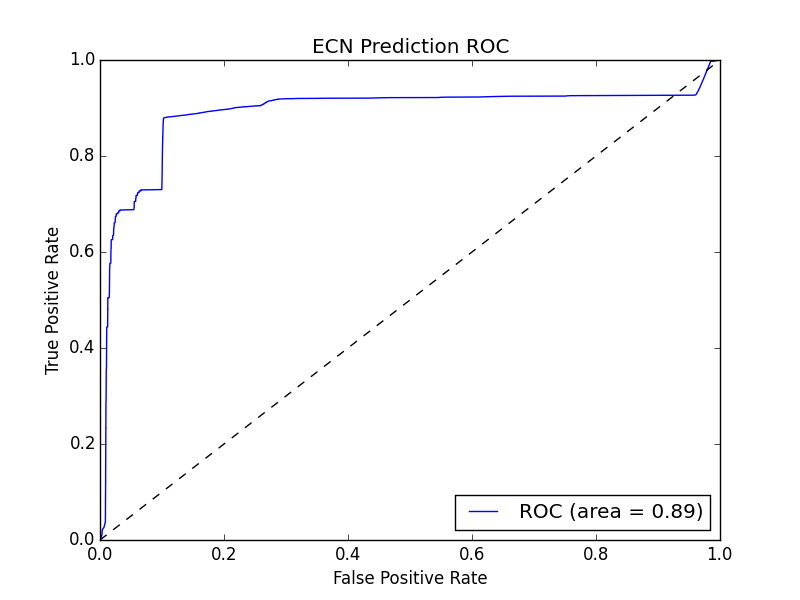
\includegraphics[width=10cm]{LRRoc.png}
\caption{ROC curve of Logistic Regression classifier}
\label{LRRoc}
\end{figure}




\par Next we applied Decision Tree algorithm and regulated the maximum depth of the tree to be $5$ and the minimum samples in each leaf node to be $10000$ to avoid overfitting. Figure. \ref{DecisionTreeRoc} gives the ROC curve of Decision Tree Classifier. The area under ROC curve is $0.98$. This indicates excellent ($0.90 - 1$) prediction result. The feature importance are given as [$0.011703$, $0.00085$, $0.000000$, $0.03985$, $0.94760$] for [$T_{s_{i}}$, $T_{r_{i}}$, send\_ewma, receive\_ewma, rtt\_ratio], from which we can conclude that rtt\_ratio is the most important feature to predict congestion. 
%\begin{figure}
%\centering
%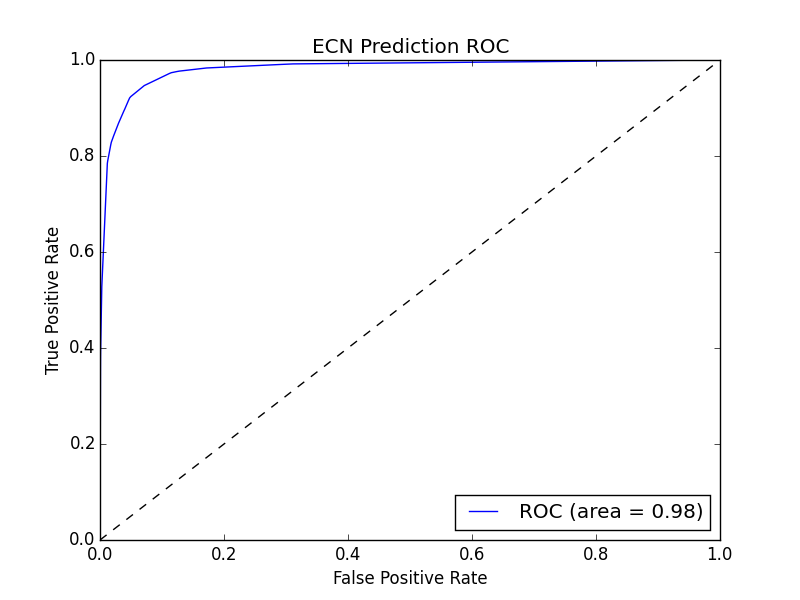
\includegraphics[width=10cm]{DecisionTreeRoc.png}
%\caption{ROC curve of Decision Tree Classifier (max\_depth = 5, min\_samples\_leaf = 10000)}
%\label{DecisionTreeRoc}
%\end{figure}

\begin{figure}[!htb]\centering
   \begin{subfigure}{0.49\textwidth}
     \frame{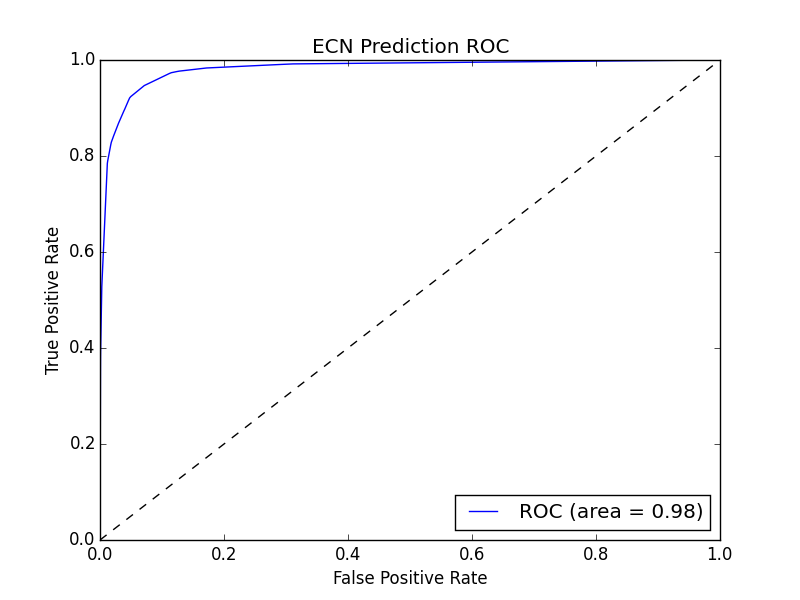
\includegraphics[width=6cm]{DecisionTreeRoc.png}}
\caption{max\_depth = 5, min\_samples\_leaf = 10000}
\label{DecisionTreeRoc}

   \end{subfigure}
   \begin {subfigure}{0.49\textwidth}
     \frame{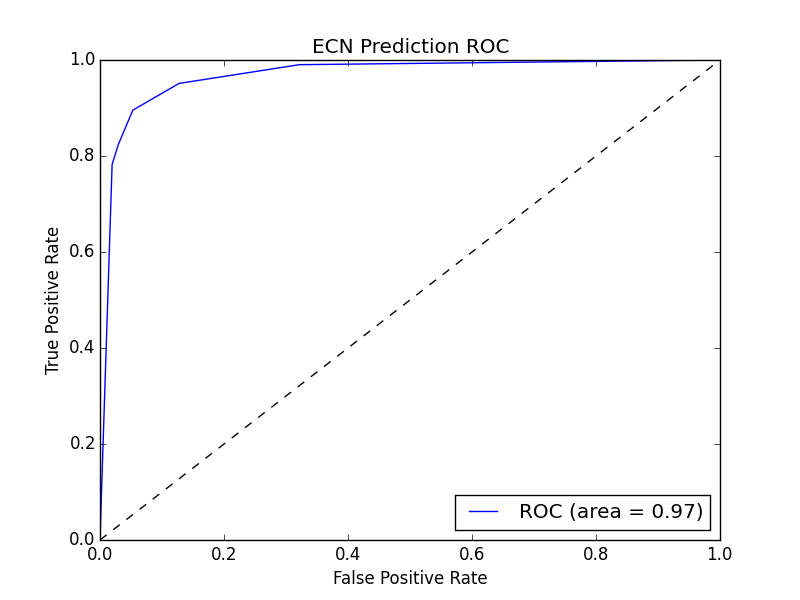
\includegraphics[width=6cm]{DTRoc.png}}
\caption{max\_depth = 3, min\_samples\_leaf = 100000}
\label{DTRoc}
   \end{subfigure}
   \caption{ROC curve of Decision Tree classifier}
\label{fig:roc1}
\end{figure}
Further we changed the maximum depth to $3$ and minimum samples of each leaf node to $100000$, the ROC is displayed in Figure. \ref{DTRoc}. The feature importance becomes [$0$, $0$, $0$, $0$, $1$]. This indicates the decision tree is doing the binary classification merely based on rtt\_ratio. All other features are not contributed to the binary classification process. 
%\begin{figure}
%\centering
%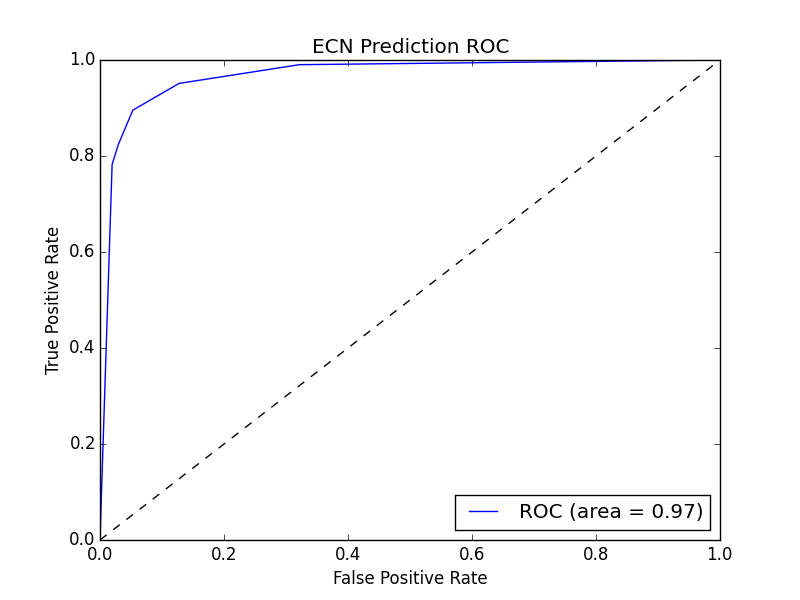
\includegraphics[width=10cm]{DTRoc.png}
%\caption{ROC curve of Decision Tree Classifier (max\_depth = 3, min\_samples\_leaf = 100000)}
%\label{DTRoc}
%\end{figure}
The decision tree is shown in Figure. \ref{DT}. In Figure. \ref{DT}, X[4] is rtt\_ratio, the first layer is classified by this feature. The cumulative density function (CDF) of rtt\_ratio is given in Figure. \ref{CDFrtt}. The blue line is the CDF curve of rtt\_ratio when congestion is experienced while the red line is when congestion is not experienced. Take $1.2$ as an example, the probability of rtt\_ratio to be less than $1.13$ is $82\%$ when there is no congestion. However, that probability is approximately $0\%$ when congestion experienced. This is consistent with the result of feature importance generated from Decision Tree algorithm. 

\begin{figure}
\centering
  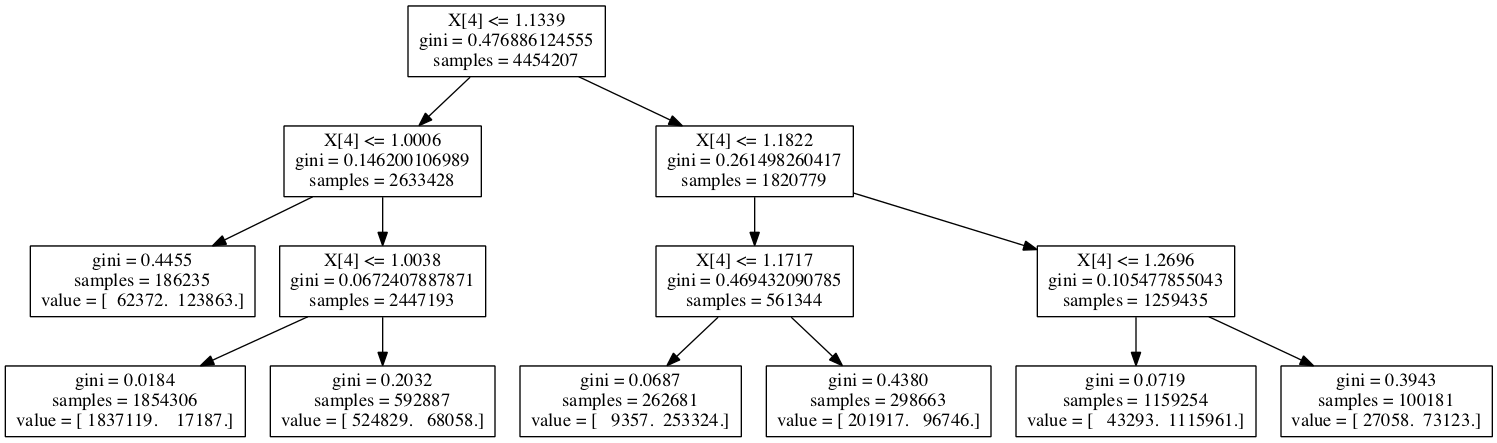
\includegraphics[width=\textwidth,height=4cm]{tree.png}
  \caption{Decision Tree (max\_depth = 3, min\_samples\_leaf = 100000)}
  \label{DT}
\end{figure}

\begin{figure}[!htb]\centering
   \begin{subfigure}{0.49\textwidth}
     \frame{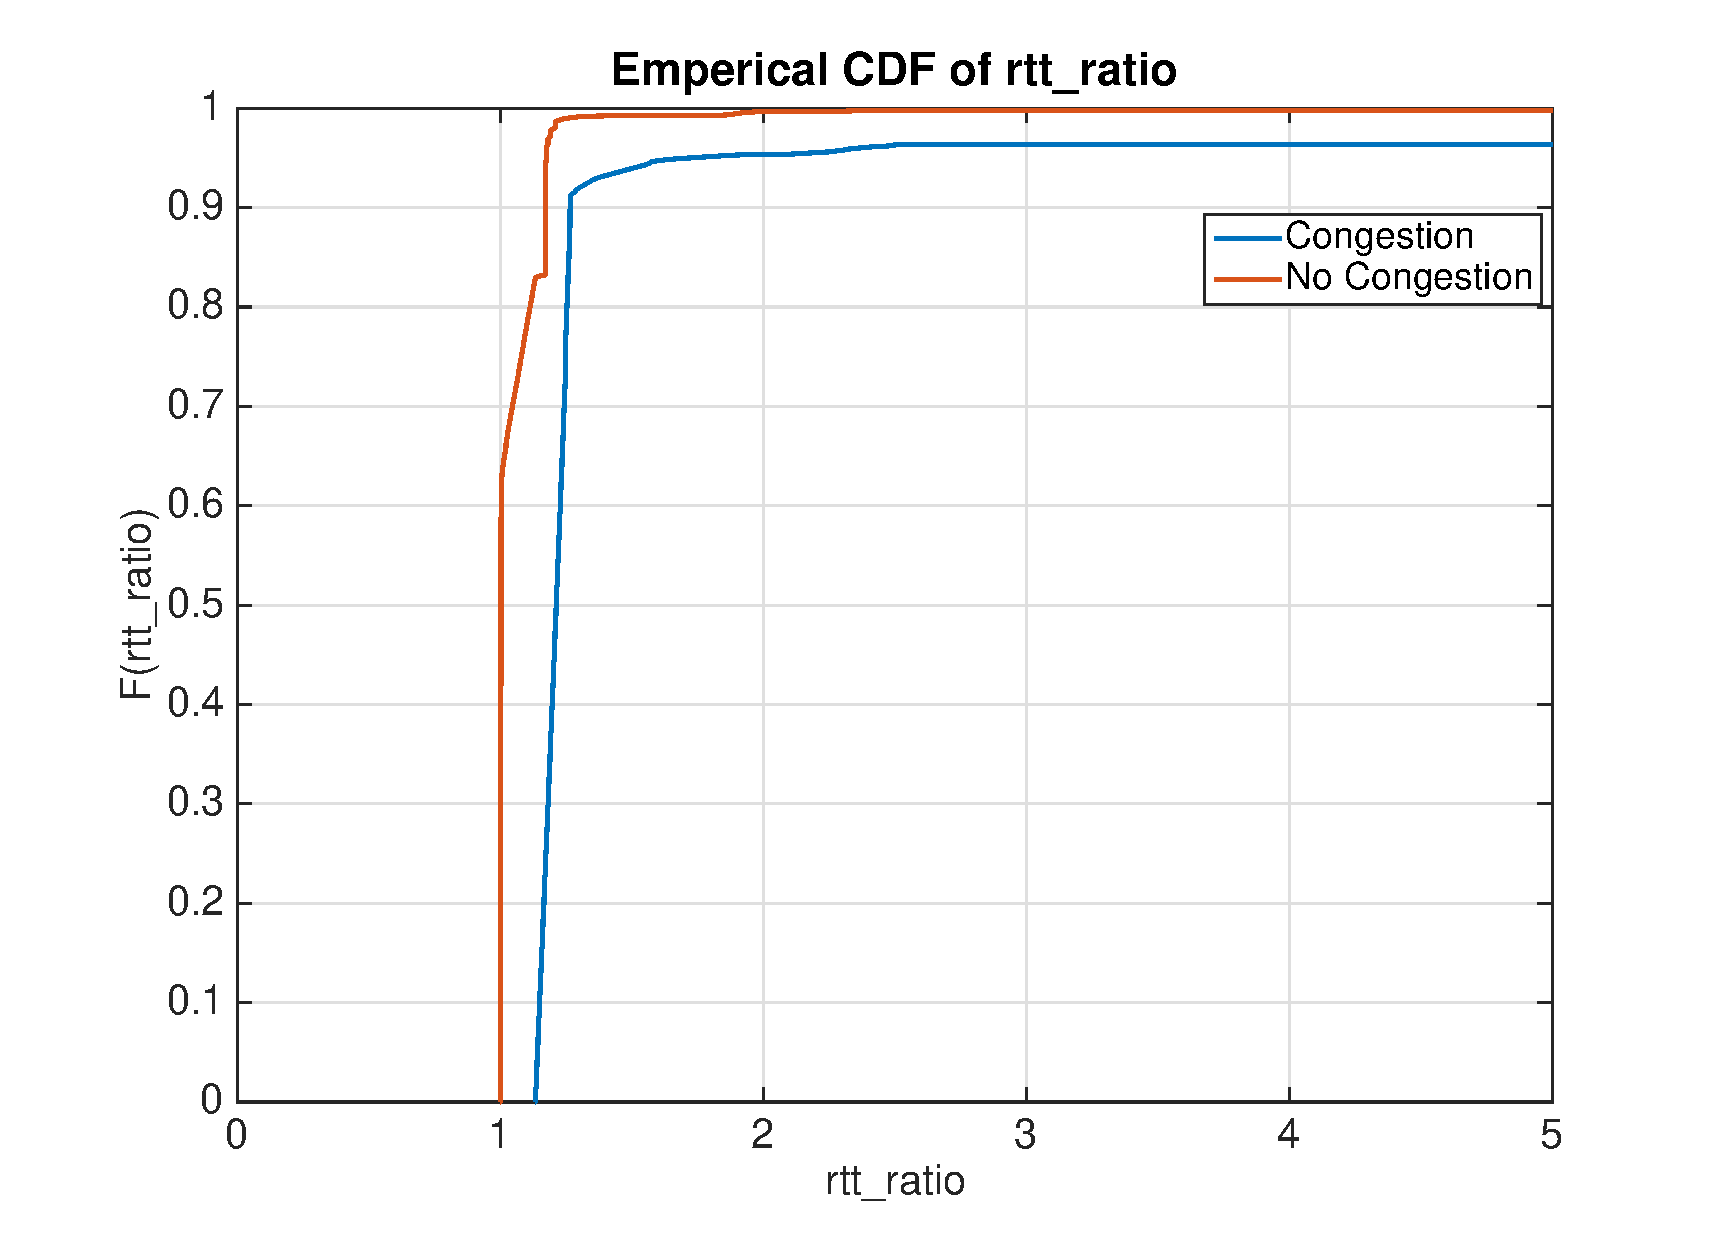
\includegraphics[width=6cm]{cdfrtt1.eps}}
\caption{CDF of rtt\_ratio with same propagation delay}
\label{CDFrtt}

   \end{subfigure}
   \begin {subfigure}{0.49\textwidth}
     \frame{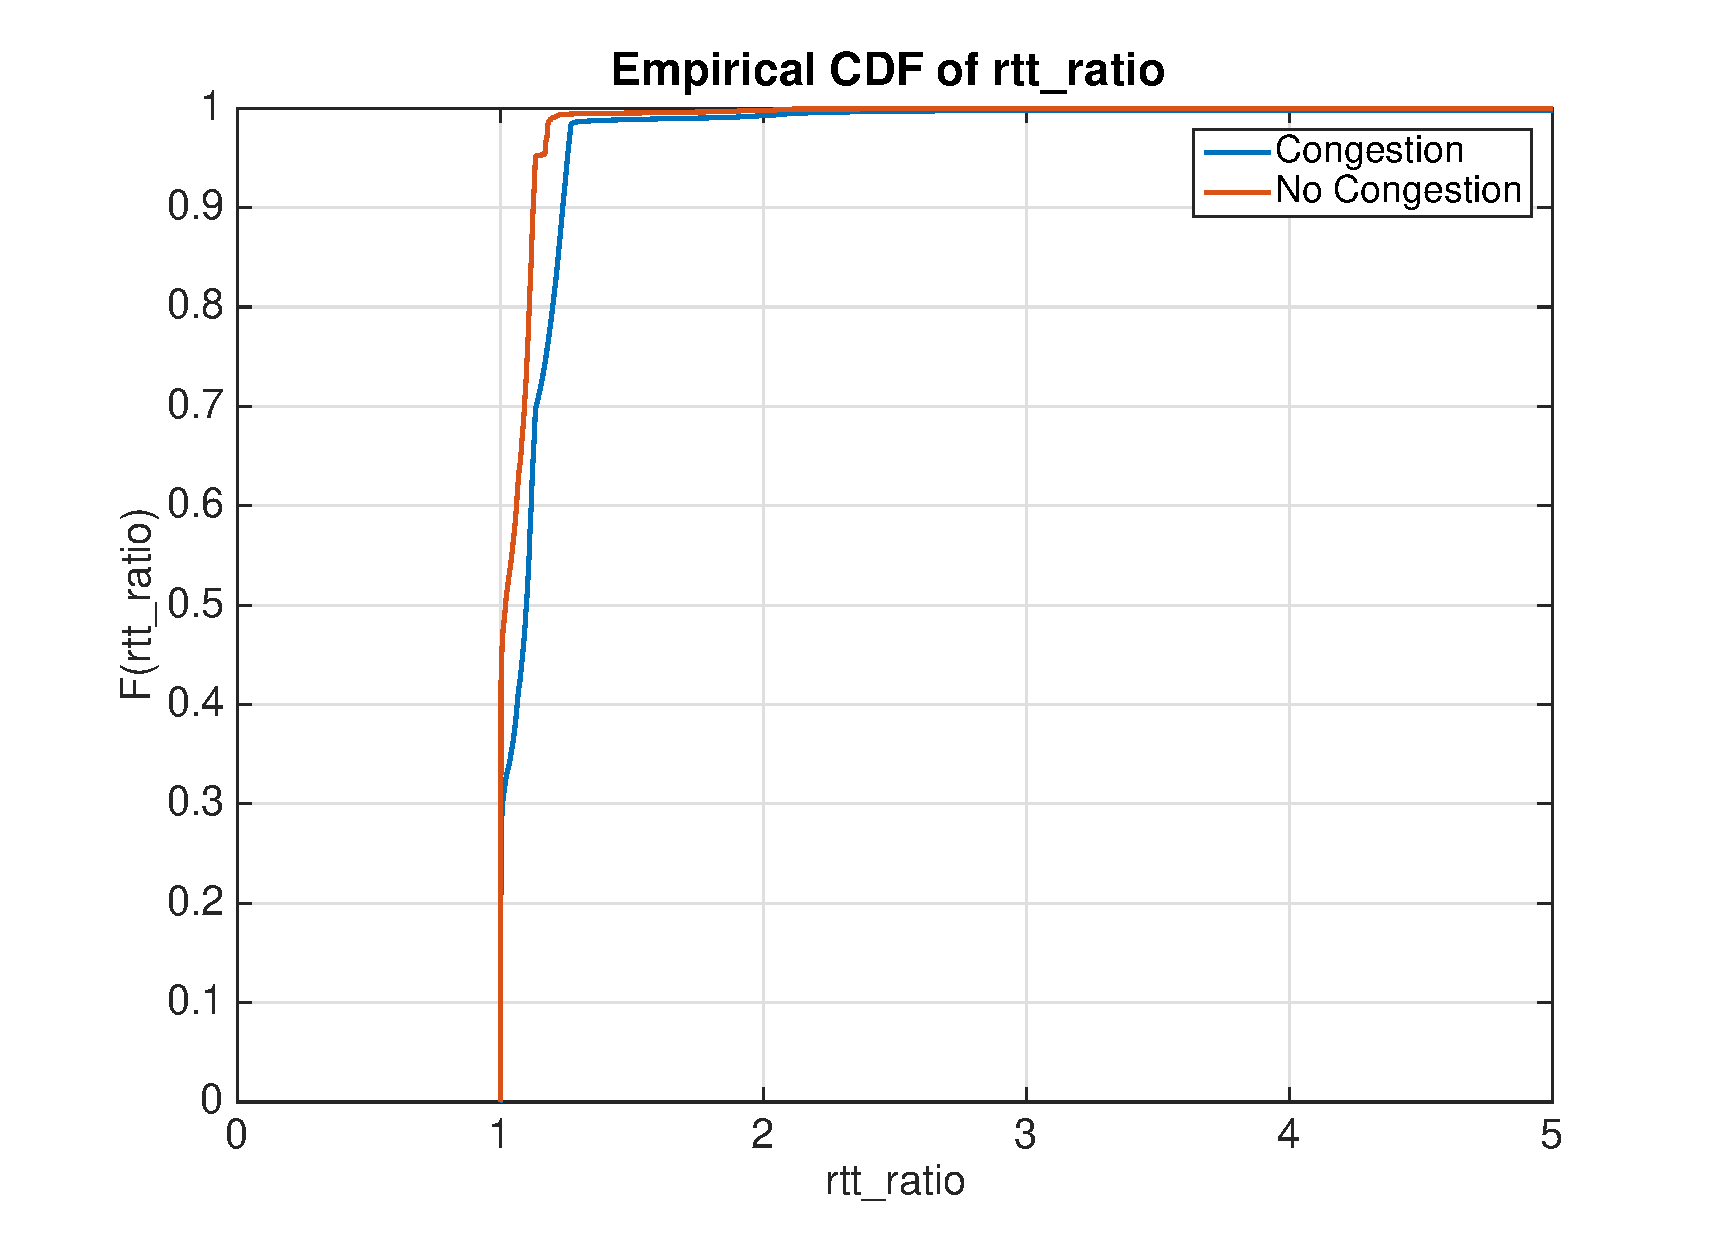
\includegraphics[width=6cm]{cdfrtt2.eps}}
\caption{CDF of rtt\_ratio with different propagation delay}
\label{CDFrttDiff}
   \end{subfigure}
\caption{CDF of rtt\_ratio}
\label{fig:cdf1}
\end{figure}



%\begin{figure}
%\centering
%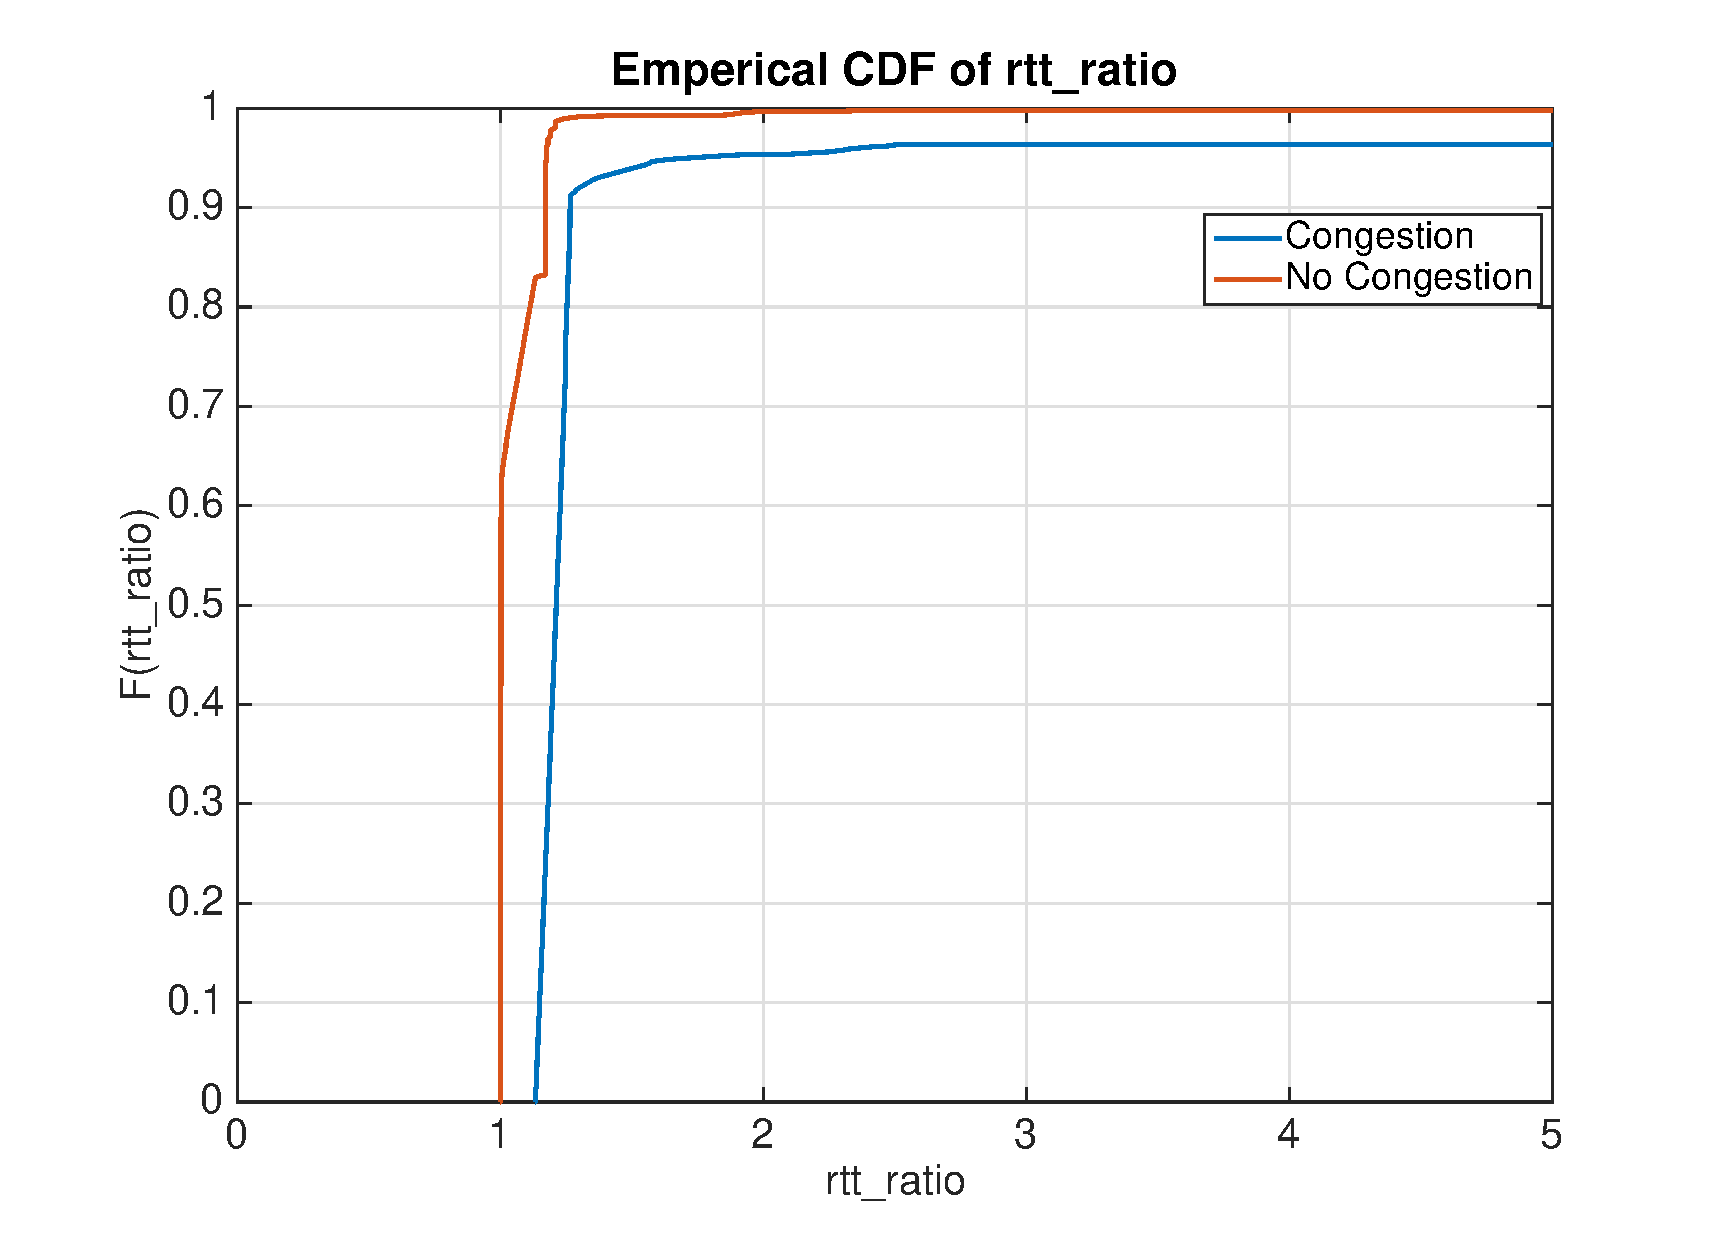
\includegraphics[width=10cm]{cdfrtt1.eps}
%\caption{CDF of rtt\_ratio}
%\label{CDFrtt}
%\end{figure}

\par The above results are generated from a network with fixed propagation delay. To learn how this prediction algorithm works when network condition changes, we investigated Scenario 1 and 2 with variations of propagation delay. We simulated networks with access delay and queue capacity as in TABLE \ref{tab:varyRTT}.
\begin{table}
\begin{center}
\caption {Simulation Parameters} \label{tab:varyRTT}
\begin{tabular}{ |c|c| }
 \hline
 Access Link Delay & 5ms, 10ms, 20ms  \\
 \hline
 BottleNeck Link Delay & 10ms, 20ms, 40ms\\
 \hline
 Queue Capacity & Delay-Bandwidth Product\\
 \hline
\end{tabular}
\end{center}
\end{table}
The Logistic Regression algorithm generated the ROC curve as in Figure. \ref{LRROCDiff}. The area under ROC curve is $0.654497$, which indicates poor performance ($0.60-0.70$). The decision boundary is $ -0.46605323*f_{1} - 7.33485574*f_{2} - 0.34620622
*f_{3} - 1.41154115*f_{4} + 5.20171832*f_{5} - 5.53557771 = 0$. The coefficient of each feature follows the same pattern as before. Decision Tree classifier is then applied to the collected dataset. The ROC curve is as in Figure. \ref{DTROCDiff}. The area under ROC curve is $0.701188$, which is on the boundary of poor performance. The feature importance is [$0.000955787581$, $0.000389816495$, $0.00489484823$, $0.0636899225$, $0.930069625$]. This is consistent with the previous result that rtt\_ratio is the most important feature. Those two figures indicate that when network condition changes, the predictability of congestion from the aforementioned five features decreases. Figure. \ref{CDFrttDiff} shows the CDF of rtt\_ratio with different link propagation delay. The figure indicates near $30\%$ overlap of the CDF curve of Congestion Experience packet and No Congestion packet. This again verifies the prediction results.
\begin{figure}[!htb]\centering
\begin{subfigure}{0.49\textwidth}
\frame{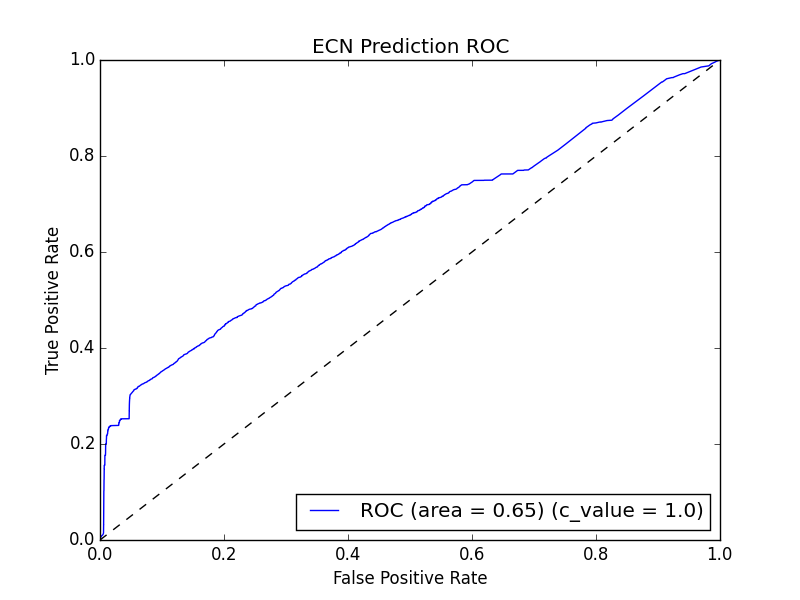
\includegraphics[width=7cm]{LRRocDiffProp.png}}
\caption{ROC curve of Logistic Regression classifier with different propagation delay}
\label{LRROCDiff}
\end{subfigure}
\begin{subfigure}{0.49\textwidth}
\frame{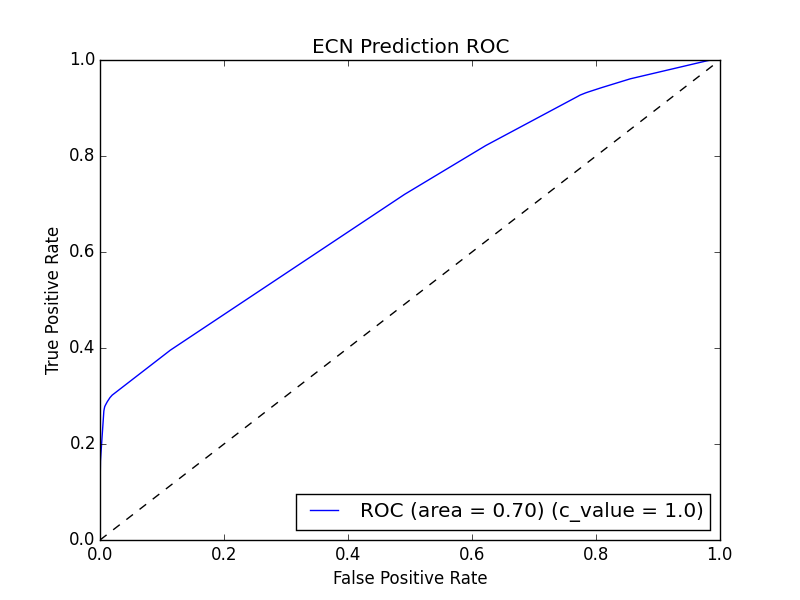
\includegraphics[width=7cm]{DTRocDiffProp.png}}
\caption{ROC curve of Decision Tree classifier with different propagation delay}
\label{DTROCDiff}
\end{subfigure}
\caption{ROC curves with different propogation delay}
\label{fig:roc2}
\end{figure}
%\begin{figure}
%\centering
%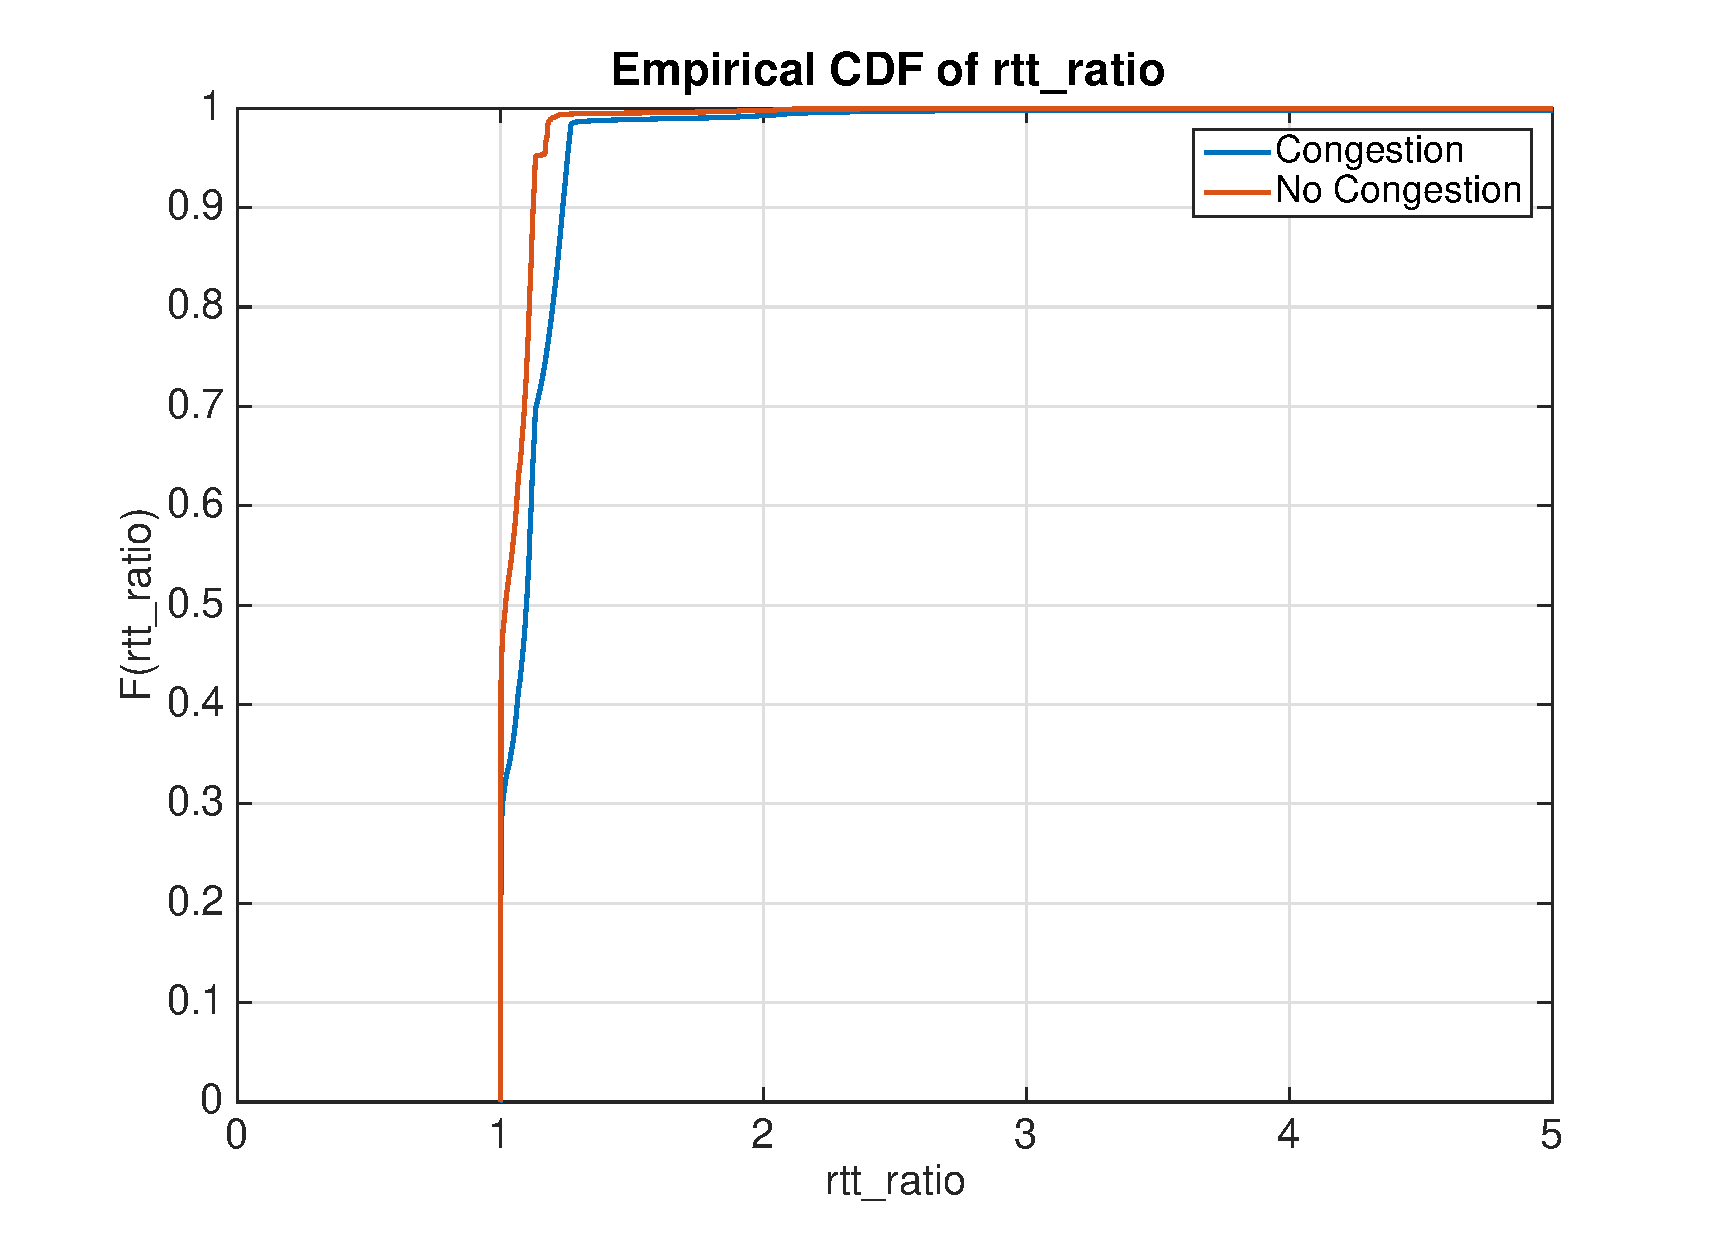
\includegraphics[width=10cm]{cdfrtt2.eps}
%\caption{CDF of rtt\_ratio with Different Propagation Delay}
%\label{CDFrttDiff}
%\end{figure}




\section{Chapter Summary}
\label{Conclusions and Future Work}
In this chapter, we proposed a data driven machine learning congestion detection algorithm. Datasets are collected using NS2 for a dumbbell model with five different traffic scenarios. Five features are formatted from end user data. When the network condition is not changing, which means the propagation delay of each link is stable, our algorithm can detect congestion with high precision from the five features. In contrast, if the network condition changes, the algorithm fails to work. In both cases, rtt\_ratio is the most important feature to predict congestion. Other four features are less useful when doing the binary classification. The area under ROC curve is consistent with the CDF of rtt\_ratio. For stable network, a fast reacting congestion control algorithm can be designed based on our congestion detection algorithm for 5G mmWave communication network.
